\documentclass[../main.tex]{subfiles}
\begin{document}

\chapter{Optical analysis of Mrk 783}
\label{cap:paper3}

In this chapter I will report the results of the optical follow-up of Mrk 783, the NLS1 galaxy with radio extended emission analyzed in the previous chapter.
I acquired new spectroscopic data in order to investigate the presence of an extended narrow-line region (ENLR) aligned with the radio emission.

The new data revealed the presence of an ENLR with a maximum size of $38\,\si{kpc}$, well above the typical size of these extended structures at $z<0.1$.
The diagnostic diagrams confirm that the gas is ionized by the AGN continuum, at least in the inner kiloparsecs where all the emission lines were detected.

The analysis of the spectra, together with new and archival broad-band images, suggests that the galaxy recently merged with a companion and that it might be in the first stages of the interaction with another companion source located $\sim 100\,\si{kpc}$ away. 

\section{Introduction}
\label{sec:pap3_intro}

The extended narrow-line region (ENLR) is one of the most puzzling and less studied structures observed in active galactic nuclei (AGN).
It is a region of highly ionized gas that can have an extension, usually traced thanks to optical emission lines, of the order of tens of kiloparsecs \citep[e.g.][]{Stockton87,Tadhunter89,Keel12}.

ENLRs are observed both in Type 1 and Type 2 AGN (mainly in Seyfert galaxies), even though they seem to have different properties in the two samples.
In Seyfert 2s the ENLR is usually characterized by a conical or bi-conical shape with the apexes pointing toward the nucleus of the galaxy (for this reason ENLRs are often called \emph{ionization cones}), while Seyfert 1s usually show more compact and halo-like structures \citep{Schmitt03,Schmitt03b}.

This behaviour can be explained thanks to the Unified Model of AGN \citep{Antonucci93,Urry95}.
According to this model, the core of the AGN is surrounded by a dusty torus, which is able to absorb part of the ionizing radiation produced in the inner region of the nucleus.
The radiation, therefore, can escape only along the torus axis and photo-ionize the surrounding gas, creating the NLR.
If the ionizing radiation can escape the NLR and it finds gas at larger radii it will produce the ENLR.

Since Type 1 AGN are observed close to face-on, the line of sight falls inside the cone, producing the halo-like shape observed in these objects, while in Seyfert 2s the AGN is observed almost edge-on, allowing the observation of the full extension of the structure and its conical shape \citep{Schmitt03,Schmitt03b}.
This property makes ionization cones one of the best proxy to measure the inclination of the AGN with respect to the line of sight \citep{Fischer13,Marin14}.

The second factor influencing the presence and the shape of the ENLR is the galactic scale gas distribution. 
A spherical distribution of host galaxy gas would allow the formation of ionization cones only on Type 2 AGN, while a disk distribution would allow to observe these shapes also in Type 1 objects \citep{Mulchaey96b,Schmitt03b}.
Ionization cones are, indeed, observed in several Type 1 AGN (e.g. NGC\,4151, \cite{Pogge88}; Mrk\,79, \cite{Schmitt03}).
New results from \citet{He18} suggest that $30$--$40\%$ of AGN with ENLR are Type 1 objects. 

The ENLR is often characterized by a spectrum with complex lines profile showing double peaks or asymmetries \citep{Dietrich98,Morganti07,Ozaki09,Congiu17b}, produced by the presence of several kinematic components in the gas.
In some galaxies, outflows of gas with velocities of $400$ -- $600\,\si{\kms}$ have been observed in several gas phases (from the cold molecular gas to the warm ionized one) inside the ionization cones \citep[e.g. IC\,5063,][]{Baldwin87,Morganti98,Morganti07,Dasyra15,Morganti15}.
Moreover ionization cones seem to be often aligned to the radio jets of the AGN \citep{Unger87,Nagar99,Schmitt03,Schmitt03b} and in some case it has been proved that shocks can be important in the ionization of the ENLR gas \citep{Congiu17b,Rodriguez17}.
All these properties might be explained as the result of the interaction between the ISM of the galaxy and the radio jet of the AGN \citep[e.g.][]{Unger87,Tadhunter14,Congiu17b,Rodriguez17}.

With this mind, soon after the discovery of a kiloparsec scale radio emission in the narrow-line Seyfert 1 (NLS1) galaxy Mrk\,783 \citep{Congiu17}, I started an optical follow-up of the source which brought to the discovery of a very extended optical emission at the same position angle (PA) of the radio emission. 
NLS1s are a peculiar class of Type 1 AGN, classified for the first time by \citet{Osterbrock85}.
They are characterized by narrow permitted emission lines, full width at half maximum (FWHM) of $\Hb$ $<2000\,\si{\kms}$, [\ion{O}{III}]$\lambda5007/\Hb$ ratio $<3$ \citep{Osterbrock85} and strong iron multiplets indicating that they are type 1 AGN \citep{Goodrich89}.
The analysis of new spectra of Mrk\,783 \citep{Congiu17c} revealed that the strongest optical emission lines can be traced up to $\sim 30\,\si{arcsec}$ from the nucleus, which correspond to a projected size of $\sim 38\,\si{kpc}$, making this ENLR one of the most extended discovered so far at $z<0.1$.

In this paper I present a detailed analysis of several spectra and images of Mrk\,783 to characterize the properties of the emission, and of the host galaxy in general, and to study the relation between the ENLR and the extended radio emission.

In Sec.\,\ref{sec:pap3_mrk783} I will describe the target, Mrk\,783 while in Sec.\,\ref{sec:obs} I will present new and archival observations.
In Sec.\,\ref{sec:analysis1_pap3} I will present a qualitative analysis of all the data, while Sec.\,\ref{sec:spectral_anal} will focuse on a more quantitative and detailed analysis of the spectra.
Finally, in Sec.\,\ref{sec:pap3_discussion} I will discuss the results that will be summarized in Sec.\,\ref{sec:pap3_summary}.
In this paper I adopt the following cosmological parameters: $H_0 = 70\,\si{\kms.Mpc^{-1}}$, $\Omega_{m,0} = 0.27$ and $\Omega_{\Lambda,0} = 0.73$ \citep{Komatsu11}.

\section{Mrk 783}
\label{sec:pap3_mrk783}

Mrk 783 (RA $= 13$h $03$m $58.8$s, DEC $=16$h $24$m $28$s) is a NLS1 galaxy firstly classified by \citet{Osterbrock85} at $z = 0.0672$ \citep{Hewitt91}.
The AGN is characterized by a bolometric luminosity $L_{bol} = 3.3\times 10^{44}\,\si{erg.s^{-1}}$ and the supermassive black hole (SMBH) has a mass of $\sim 4.3\times10^{7}\,\si{M_{\odot}}$ \citep{Berton15a}.
The host has been classified as a lenticular galaxy by \citet{Petrosian07}.

The object has been observed several times in the radio band and it was detected in all the major surveys (FIRST, NVSS), but only recently \citet{Congiu17} discovered a kiloparsec scale radio emission thanks to a VLA snapshot survey carried out at $5\,\si{GHz}$ in A configuration \citep{Berton18}.
The maximum extension of the radio emission has been measured, in the tapered image, to be $14\,\si{kpc}$ and it is located along PA $= \ang{131}$ \citep{Congiu17}.
Due to the very steep in-band spectra indexes measured from the VLA images, the authors hypothesized that the extended emission is a relic due to the intermittent activity of the AGN.

On VLBI scale the object has been studied by \citet{Doi13} with the VLBA at \SI{1.7}{GHz}.
Mrk 783 appears as a point-source, without any extended emission, and with brightness temperature of $7.7\times10^7$, a sign of the non thermal origin of this emission.

\section{Observations}
\label{sec:obs}

\subsection{Spectroscopy}
\label{sec:obs_spec}

\begin{table}
    \centering
    \caption{Details of spectroscopic observations.}
    \label{tab:obs_spec}
    \small
    \begin{threeparttable}
    \begin{tabular}{lcccccccc}
    \hline
    \hline
    Date& PA & Exp.& Time & $\delta$ & $\Delta\lambda$ & RMS &Standard&Instrument\\
    & & & (s) & ($\si{\angstrom.px^{-1}}$)& ($\si{\angstrom}$)& ($\si{\angstrom}$) & &\\   
    \hline
    2017-02-22 & $\ang{131}$ & $3$ & $3600$ & $2.0$ & $8.2$ & $0.87$ & LTT 4816&LDSS-3\\
    2017-06-09 & $\ang{90}$  & $3$ & $3600$ & $2.0$ & $7.9$ & $1.50$ & EG 274&LDSS-3\\
               & $\ang{131}$ & $3$ & $3600$ & $2.0$ & $7.9$ & $0.52$ & EG 274&LDSS-3\\
    2018-06-11 & $\ang{333.5}$ & $3$ & $2700$& $2.7$ &$10.04$&-&-& DOLORES\\
    \hline
    \end{tabular}
    \normalsize
    \begin{tablenotes}
    \item From left to right: (1) date of the observation, (2) position angle, (3) number of exposures per pointing, (4) total exposure time, (4) dispersion of the spectra, (5) resolution of the spectrum measured from the calibration lamp spectruma, (6) error on the wavelength calibration measured on the sky lines, (7) standard star used for flux calibration, (8) instrument used.
    \end{tablenotes}
    \end{threeparttable}
\end{table}


\begin{figure}
\centering
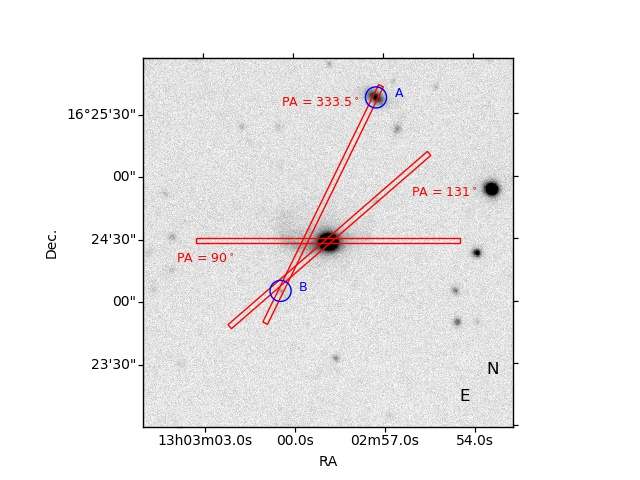
\includegraphics[width=0.8\textwidth]{images/paper3/finding.jpg} 
\caption[]{Image of Mrk 783 acquired with the Copernico telescope of the Asiago Astronomical Observatory with a g filter. In the image is shown the position of the slit during the spectroscopic observations and the position of the sources A and B observed with TNG.}
\label{fig:finding_chart}
\end{figure}

The galaxy has been observed two times with the Low Dispersion Survey Spectrograph - 3 (LDSS-3) of the Magellan telescopes.
All the observations have been performed in long slit mode, with the $1"\times4'$ ``center'' slit and the VPH-All.
This combination of slit and dispersion element allows to cover almost the whole optical wavelength range ($4250$ -- $10000\,\si{\angstrom}$) with a good sensitivity.
The galaxy was observed twice at position angle PA $=\ang{131}$, with the slit parallel to the radio emission, and once at PA $=\ang{90}$, in order to observe the secondary nucleus that will be mentioned and analyzed in Sec.\,\ref{sec:2dspectra} and following.

A fourth spectrum has been acquired with the DOLORES spectrograph of the Telescopio Nazionale Galileo (TNG) using the $1.0''$ slit and the LR-B grism.
This configuration allows to obtain a low resolution spectrum (${\rm R}\sim 600$) of the whole optical wavelength range.
As it is possible to see from Fig.\,\ref{fig:finding_chart}, this last spectrum is not centered on the galaxy itself, but it has been acquired in order to study two putative companions of the AGN.
In particular, I wanted to measure the redshift of J1302+1625 and J1303+1624 (source A and B respectively, in Fig.\,\ref{fig:finding_chart}), to investigate the possibility of the two objects being part of a group with Mrk 783

The reduction of the spectra obtained with both instruments was performed with standard IRAF\footnote{http://iraf.noao.edu/} tasks.
The spectra have been trimmed, corrected for bias and flat-field and wavelength calibrated using the spectra of a HeNeAr lamp (LDSS-3) or a HgNe lamp (DOLORES).
LDSS-3 spectra have also been flux calibrated using two different standard stars for the two runs: LTT 4816 and EG 274.
Since the main goal of the TNG spectrum was to measure the redshift of the two sources, no spectroscopic standard star has been observed.
To obtain the final data the different exposures for each spectrum have been combined and the sky contribution has been subtracted from the spectra.

Before the subtraction we used the calibration lamp spectra and some sky emission lines to estimate the resolution of the science data and the reliability of the wavelength calibration.
While LDSS-3 spectra are quite well calibrated, unfortunately the sky lines of DOLORES spectrum show a systematic shift of $\sim 5\,\si{\angstrom}$.
This must be ascribed to the fact that the calibration lamp has been observed as part of the daylight calibration plan, and not immediately after the science observation.
I tried to improve this calibration using the sky lines as reference for the calibration process.
But, since the available sky lines in the spectrum are only a few and they are quite close together, the new calibration was no reliable.
Tab. \ref{tab:obs_spec} summarizes the properties of the observations.

\subsection{Imaging}
\label{sec:obs_ima}

\begin{table}
    \centering
    \caption{Details of imaging observations.}
    \label{tab:obs_image}
    \begin{threeparttable}
    \begin{tabular}{lccccc}
    \hline
    \hline
    Instrument& Filter & Exp.& Exp. time & Seeing & Surface brightness limit \\
    & & & (s) & ($\si{arcsec}$)& ($\si{mag}$)\\   
    \hline
    SDSS &\emph{u}&$1$ &$54$ &$1.4$&$23.5$\\
    SDSS &\emph{g}&$1$ &$54$ &$1.2$&$24.7$\\
    SDSS &\emph{r}&$1$ &$54$ &$1.1$&$24.1$\\
    SDSS &\emph{i}&$1$ &$54$ &$1.0$&$23.5$\\
    SDSS &\emph{z}&$1$ &$54$ &$0.9$&$22.0$\\
    AFOSC&\emph{g}&$12$&$7200$&$2.6$&$26.1$\\
    \hline
    \end{tabular}
    \begin{tablenotes}
    \item From left to right: (1) Telescope or instrument, (2) filter, (3) number of exposures per pointing, (4) total exposure time, (5) average seeing, (6) $3\sigma$ surface brightness limit of the image.
    \end{tablenotes}
    \end{threeparttable}
\end{table}

Mrk 783 has been observed in all the available bands (\emph{ugriz}) by the Sloan Digital Sky Survey (SDSS).
In particular, for this work I considered the images of the Data Release 7\footnote{\url{https://classic.sdss.org/dr7/}}.
The g-band image of Mrk 783 in particular has a measured $3\sigma$ magnitude limit of $\sim 24.7\,\si{mag}$.
In order to better detect faint structures, such as tidal tails or spiral arms that seems to be present in the SDSS images, I also acquired a new g-band data with the Copernico telescope of the Asiago Astronomical Observatory (Fig.\,\ref{fig:finding_chart}).
The galaxy has been observed for a total exposure time of $2\,\si{hr}$ divided in $12$ single $600\,\si{s}$ exposures. 
The new data have been corrected for bias and flat-field with standard IRAF tasks.
Then the scientific images have been astrometrized.
The seeing during the observations was highly variable, therefore before the combination they were all convolved with a Gaussian kernel in order to obtain an uniform seeing corresponding to the worst seeing value.
Also an airmass correction has been applied during this phase.
Tab.\,\ref{tab:obs_image} shows a summary of the properties of the above mentioned images.


\section{Preliminary Analysis}
\label{sec:analysis1_pap3}

\subsection{Two dimensional spectra}
\label{sec:2dspectra}



The first LDSS-3 spectrum of Mrk 783 was acquired on February 2017. 
The position of the slit has been chosen in order to be aligned with the axis of the radio emission discovered in \citep{Congiu17}, since its purpose was to verify the presence of optical radio emission aligned with the radio structure.

This spectrum revealed, indeed, extended emission in all the strongest emission lines ( [\ion{O}{III}]$\lambda5007$ in particular, Fig.\,\ref{fig:three_spectra}, left panel) on both sides of the AGN.
The [\ion{O}{III}]$\lambda5007$ line can be traced up to a distance of $\sim 25\,\si{arcsec}$ from the nucleus of the galaxy, which correspond to a projected distance of $\sim 32\,\si{kpc}$.
In this spectrum the emission stop sharply, because of the presence of an interruption of the slit.
For this reason another spectrum of the source at the same PA has been acquired, taking care to position the galaxy in such a way to avoid the slit support.

The $\Hb$ region of the new spectrum is shown in Fig.\,\ref{fig:three_spectra}.
As expected, the emission is slightly more extended and it reaches $\sim 30\,\si{arcsec}$ ($\sim 38\,\si{kpc}$) from the nucleus.
It is interesting to notice that, in both spectra, the emission is not continuous but, moving from the AGN outward, it gets fainter and then it re-brights.
One possibility for this behaviour might be that the most extended emission is produced by a nearby source.
From Fig.\,\ref{fig:finding_chart} it is possible to see that there actually is a faint source close to that position, source B (J1303+1624).
J1303+1624 should have been outside the slit during the observations of both spectra, but it is possible that some imprecision during the pointing caused this source to fall inside it.
This is the reason why this source was included in the TNG observations described in Sec.\,\ref{sec:environment}.
However, if the whole emission belongs to the ENLR of Mrk 783 a projected size of $\sim 38\,\si{kpc}$ would make this ENLR one of the most extended observed so far at low redshift.

The spectrum in the right panel of Fig.\,\ref{fig:three_spectra} shows the $\Hb$ region of the last LDSS-3 spectrum, acquired at PA $=\ang{90}$.
Extended emission can be observed, on both sides of the nucleus, also at this position angle.
The size of the emission in this direction is smaller, but the [\ion{O}{III}]$\lambda5007$ line can be traced up to a distance of $\sim 17.5\,\si{arcsec}$ ($\sim 23\,\si{kpc}$) from the nucleus.
In this case the emission is continuous.
An interesting property that can be observed in the right panel of Fig.\,\ref{fig:three_spectra} is that there seems to be a second continuum $\sim 1.5\,\si{arcsec}$ west with respect to the AGN, that can be better appreciated in Fig.\,\ref{fig:flux_distr}.

\begin{figure}
\centering
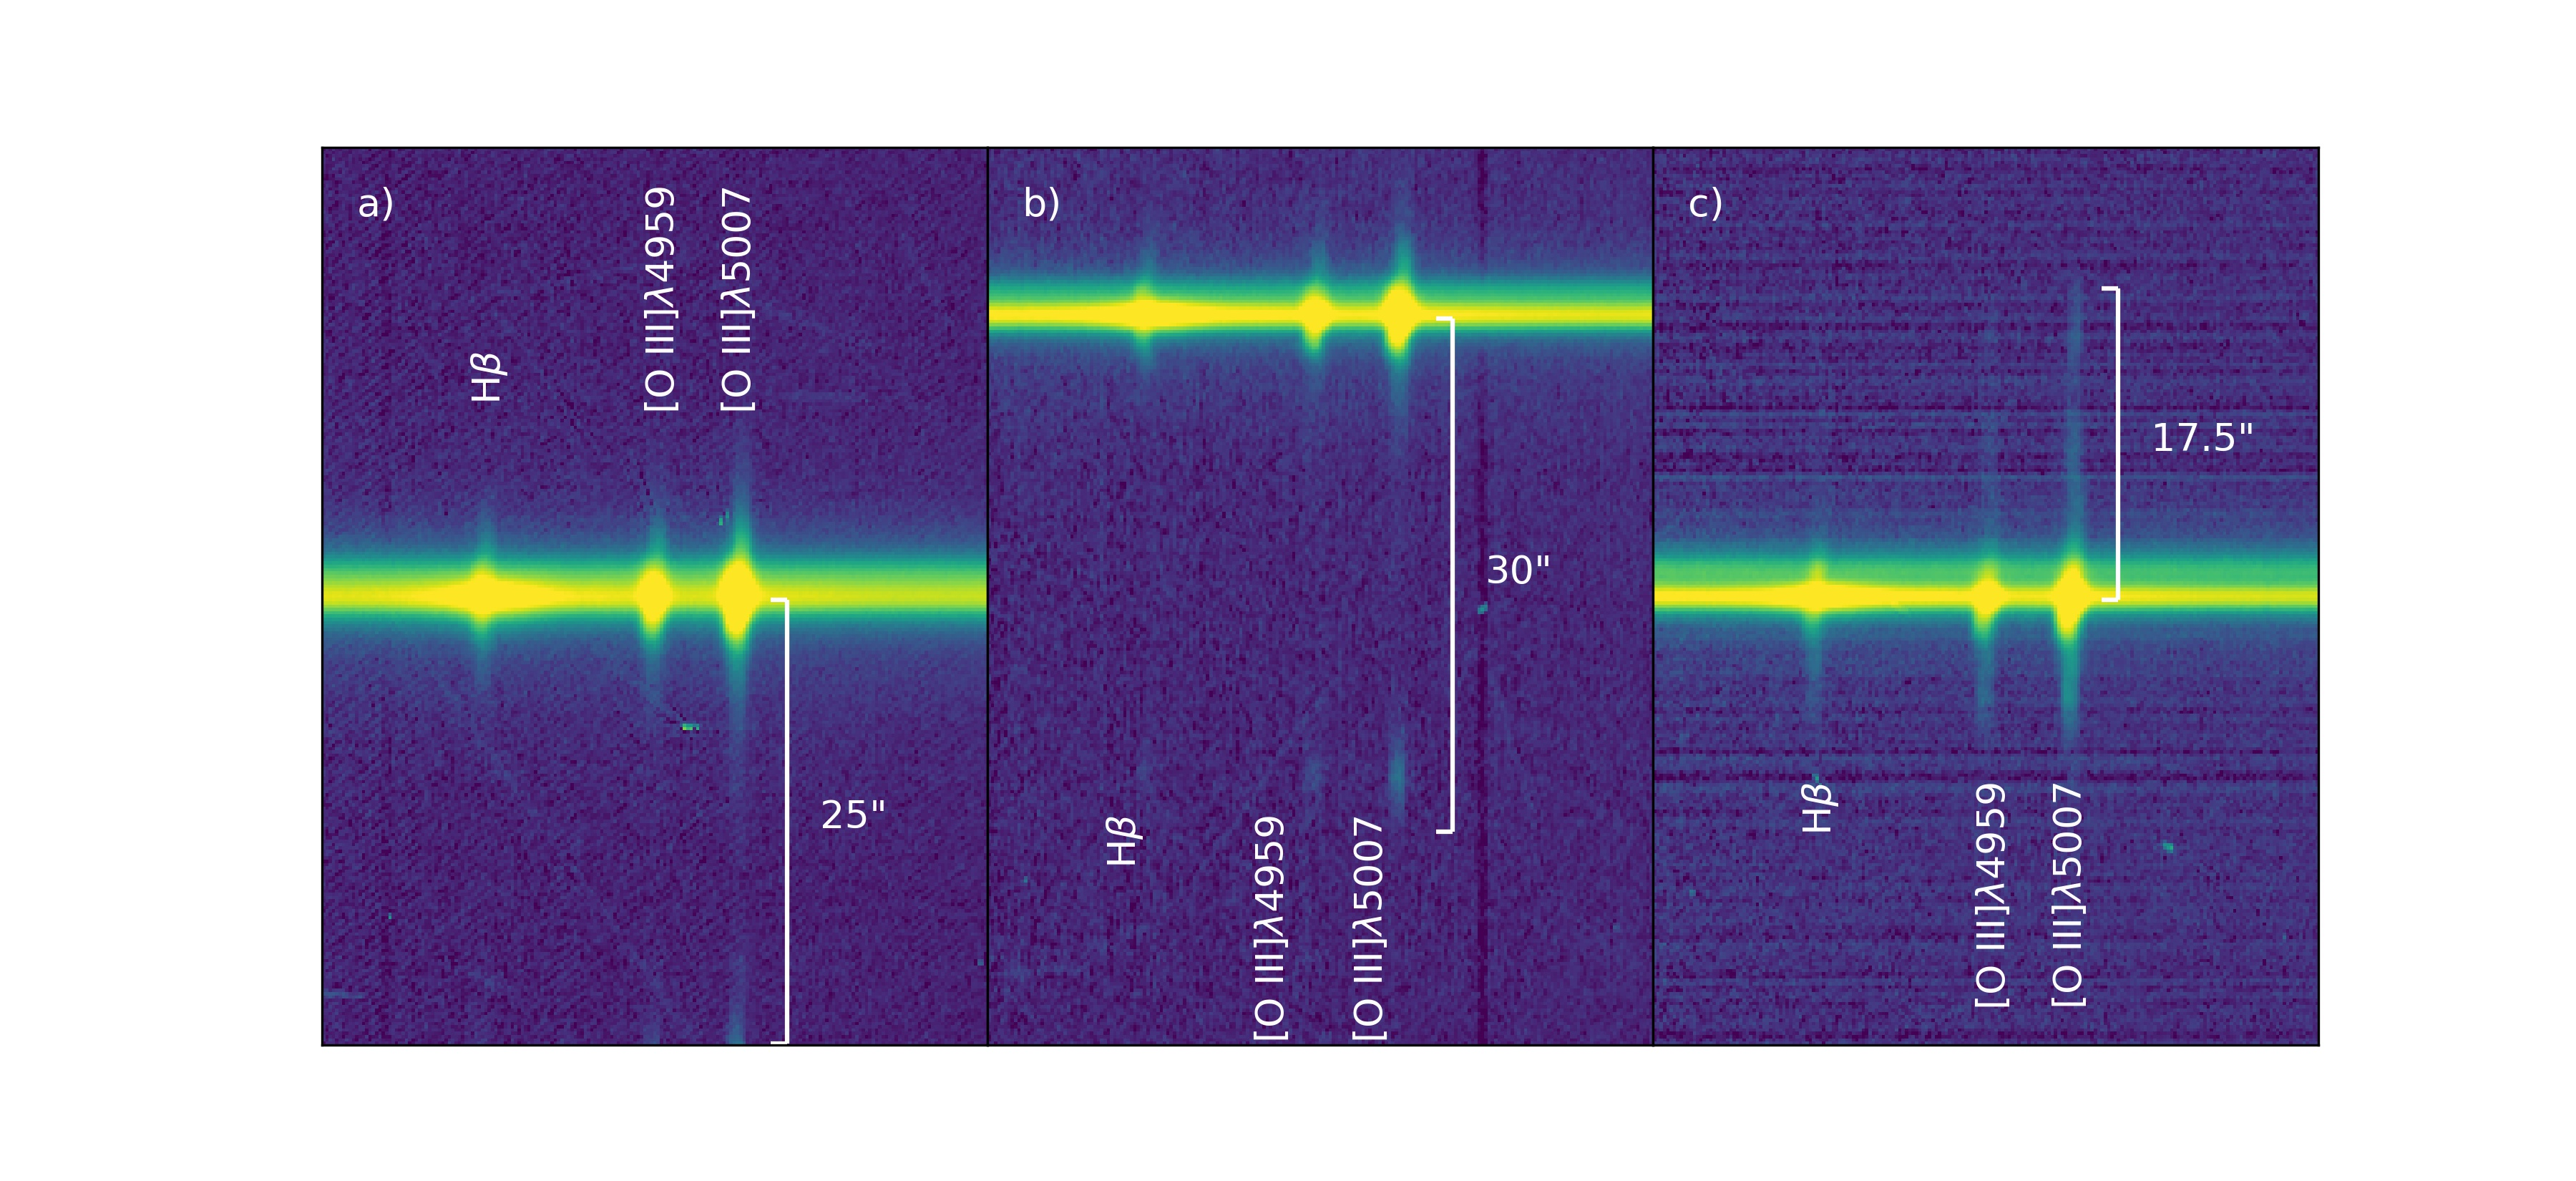
\includegraphics[width=1.1\textwidth]{images/paper3/spectra.jpg} 
\caption[]{\textbf{Panel a)} $\Hb$ region of February LDSS-3 spectrum at $\rm PA=\ang{131}$. It is possible to observe that all the three lines visible in this wavelength range ($\Hb$, [\ion{o}{iii}]$\lambda4959$ and [\ion{o}{iii}]$\lambda5007$) show extended emission that can be traced up to $\sim 25\,\si{arcsec}$ from the nucleus of the galaxy in the lower part of the image. The emission ends sharply because of an interruption of the slit. A less extended emission is present also on the other side of the nucleus. In this spectrum northwest is up and southeast is left. \textbf{Panel b)}  $\Hb$ region of June LDSS-3 spectrum at $\rm PA=\ang{131}$. The galaxy has been moved upward in the slit and the observed emission is slightly more extended, reaching $\sim 30\,\si{arcsec}$. The orientation of the spectrum is the same as in the previous panel. \textbf{Panel c)} $\Hb$ region of June LDSS-3 spectrum at $\rm PA=\ang{90}$. Extended emission is observed on both sides of the nucleus also at this PA, with the upper part reaching $\sim 17.5\,\si{arcsec}$ from the AGN. In this spectrum west is up and east is down.}
\label{fig:three_spectra}
\end{figure}


\begin{figure}
\centering
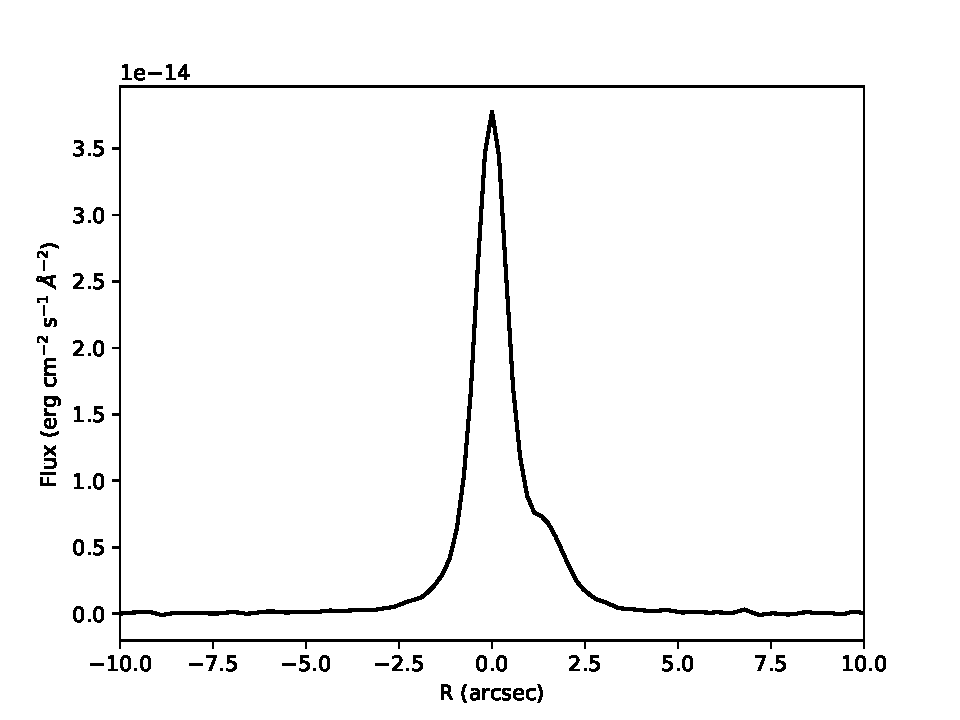
\includegraphics[width=0.8\textwidth]{images/paper3/Radial_distr.pdf} 
\caption[]{Flux distribution along the slit of the spectrum in the right panel of Fig.\,\ref{fig:three_spectra}. A single dispersion element has been considered for this plot.}
\label{fig:flux_distr}
\end{figure}



\subsection{Morphology and color}
\label{sec:morph_color}

\begin{figure}
\centering
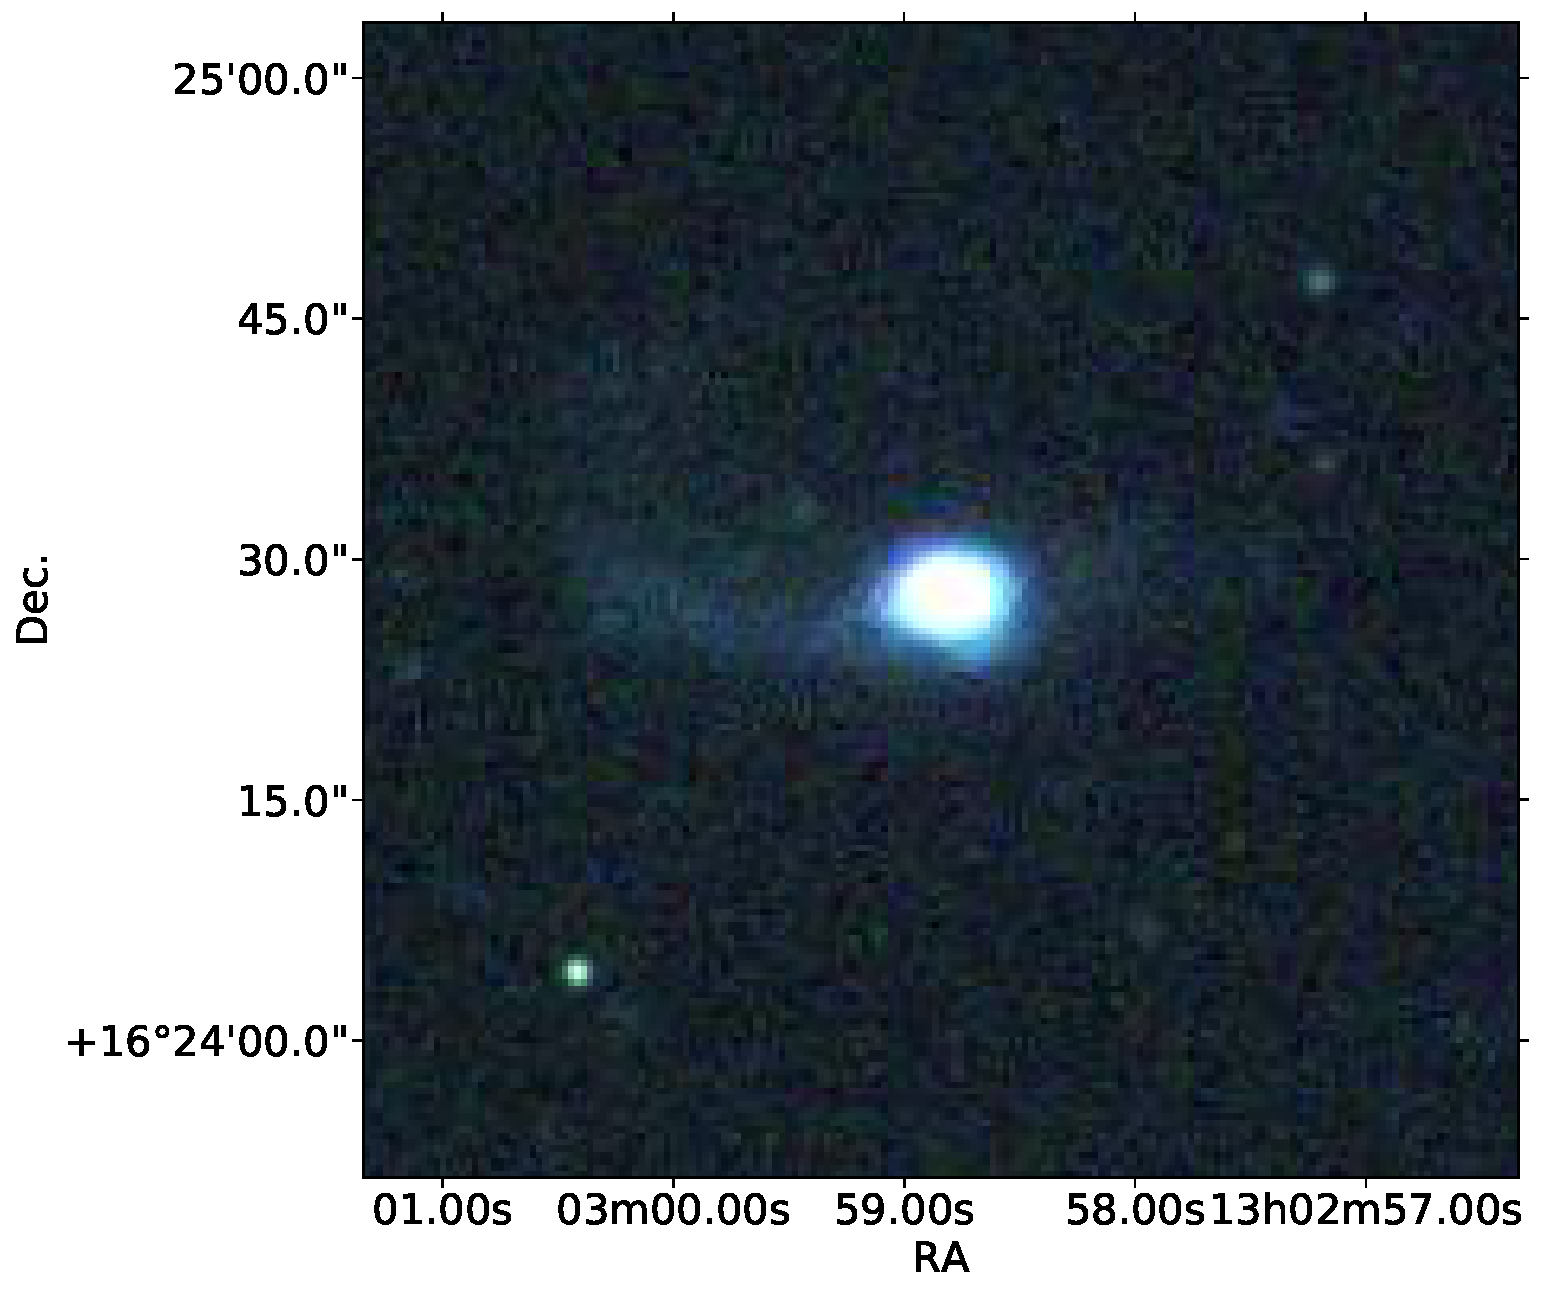
\includegraphics[width=0.7\textwidth]{images/paper3/new_rgb.pdf} %\quad
%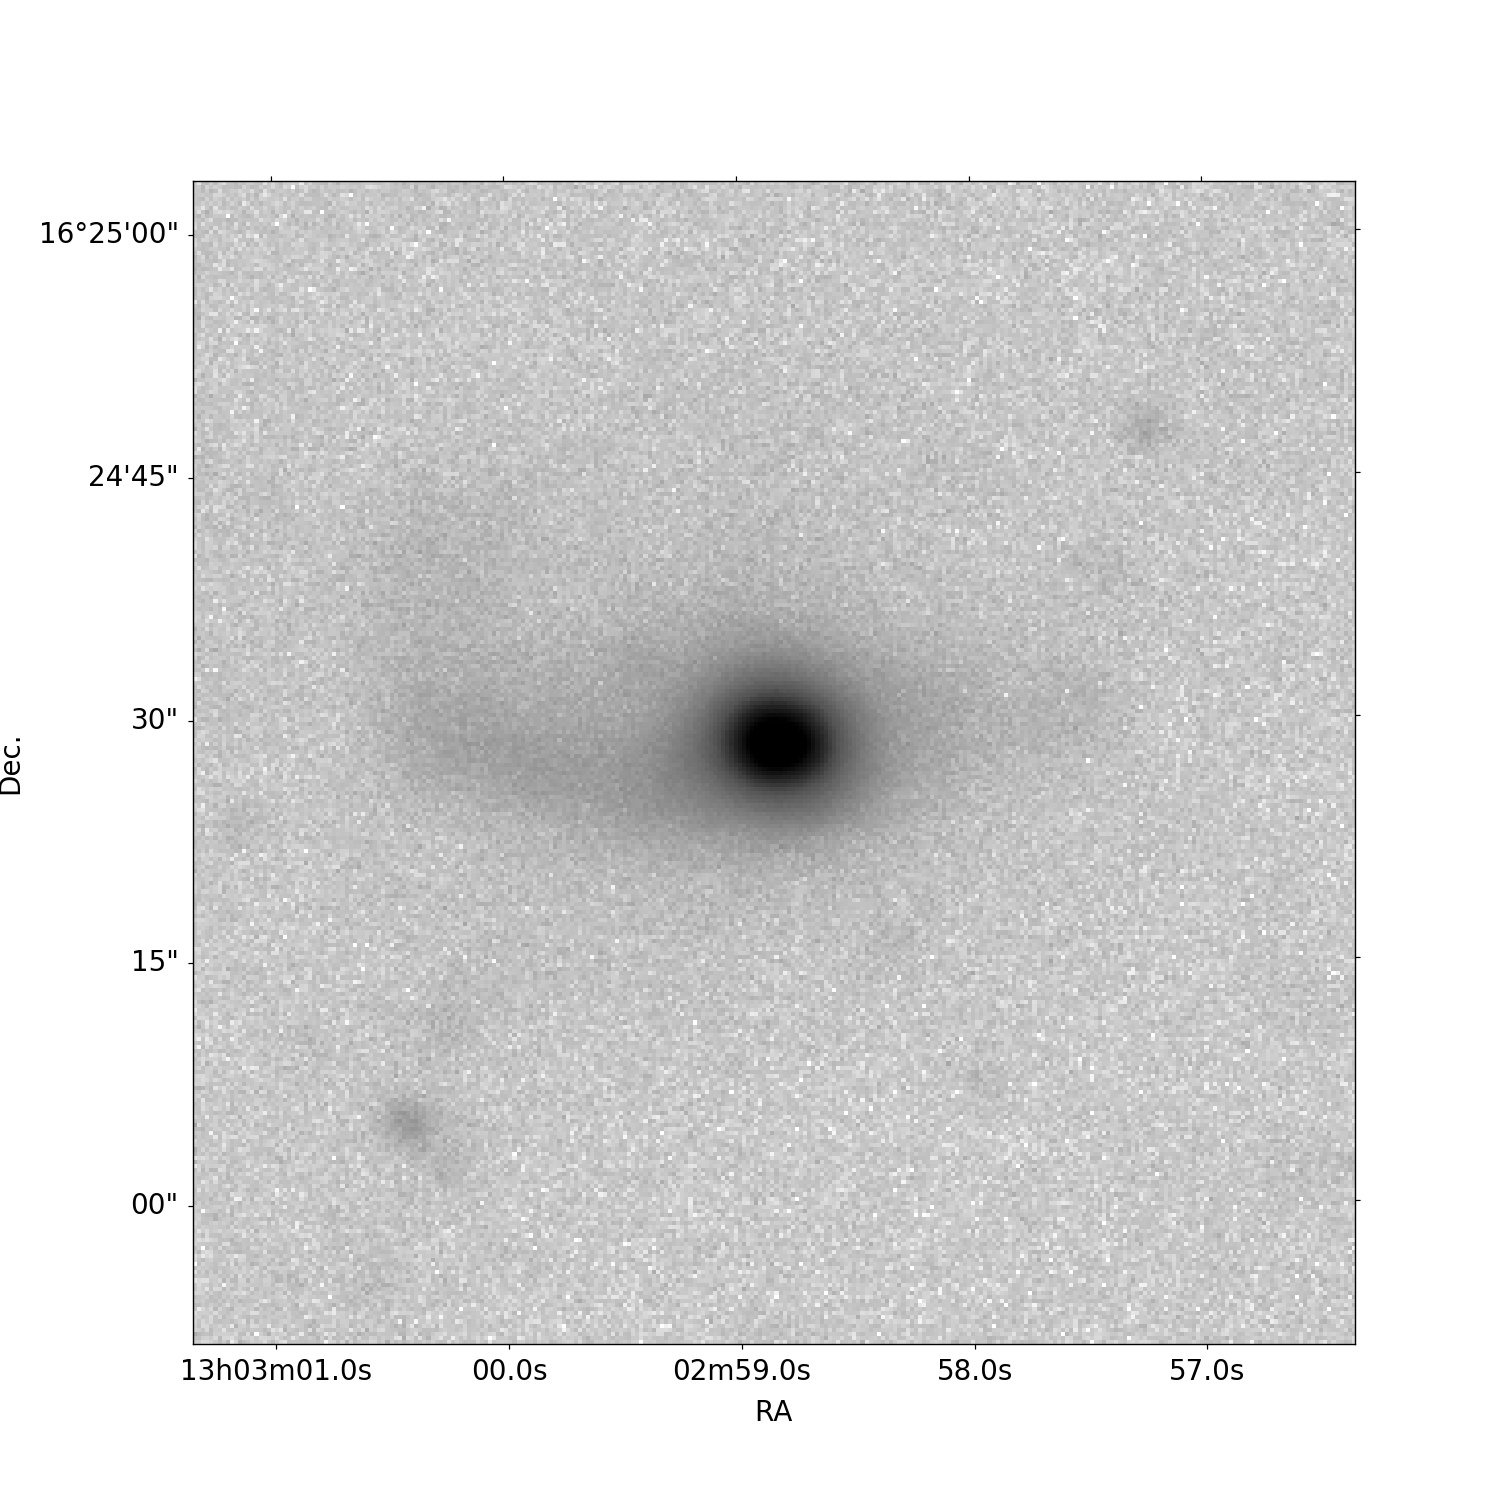
\includegraphics[width=0.45\textwidth]{images/paper3/mrk783_AFOSC.jpg}
\caption[]{\textbf{Left:} RGB image created from the \emph{g}, \emph{r} and \emph{i} SDSS images.} %\textbf{Right:} AFOSC \emph{g} image.}
\label{fig:rgb_sdss}
\end{figure} 

\begin{figure}
\centering
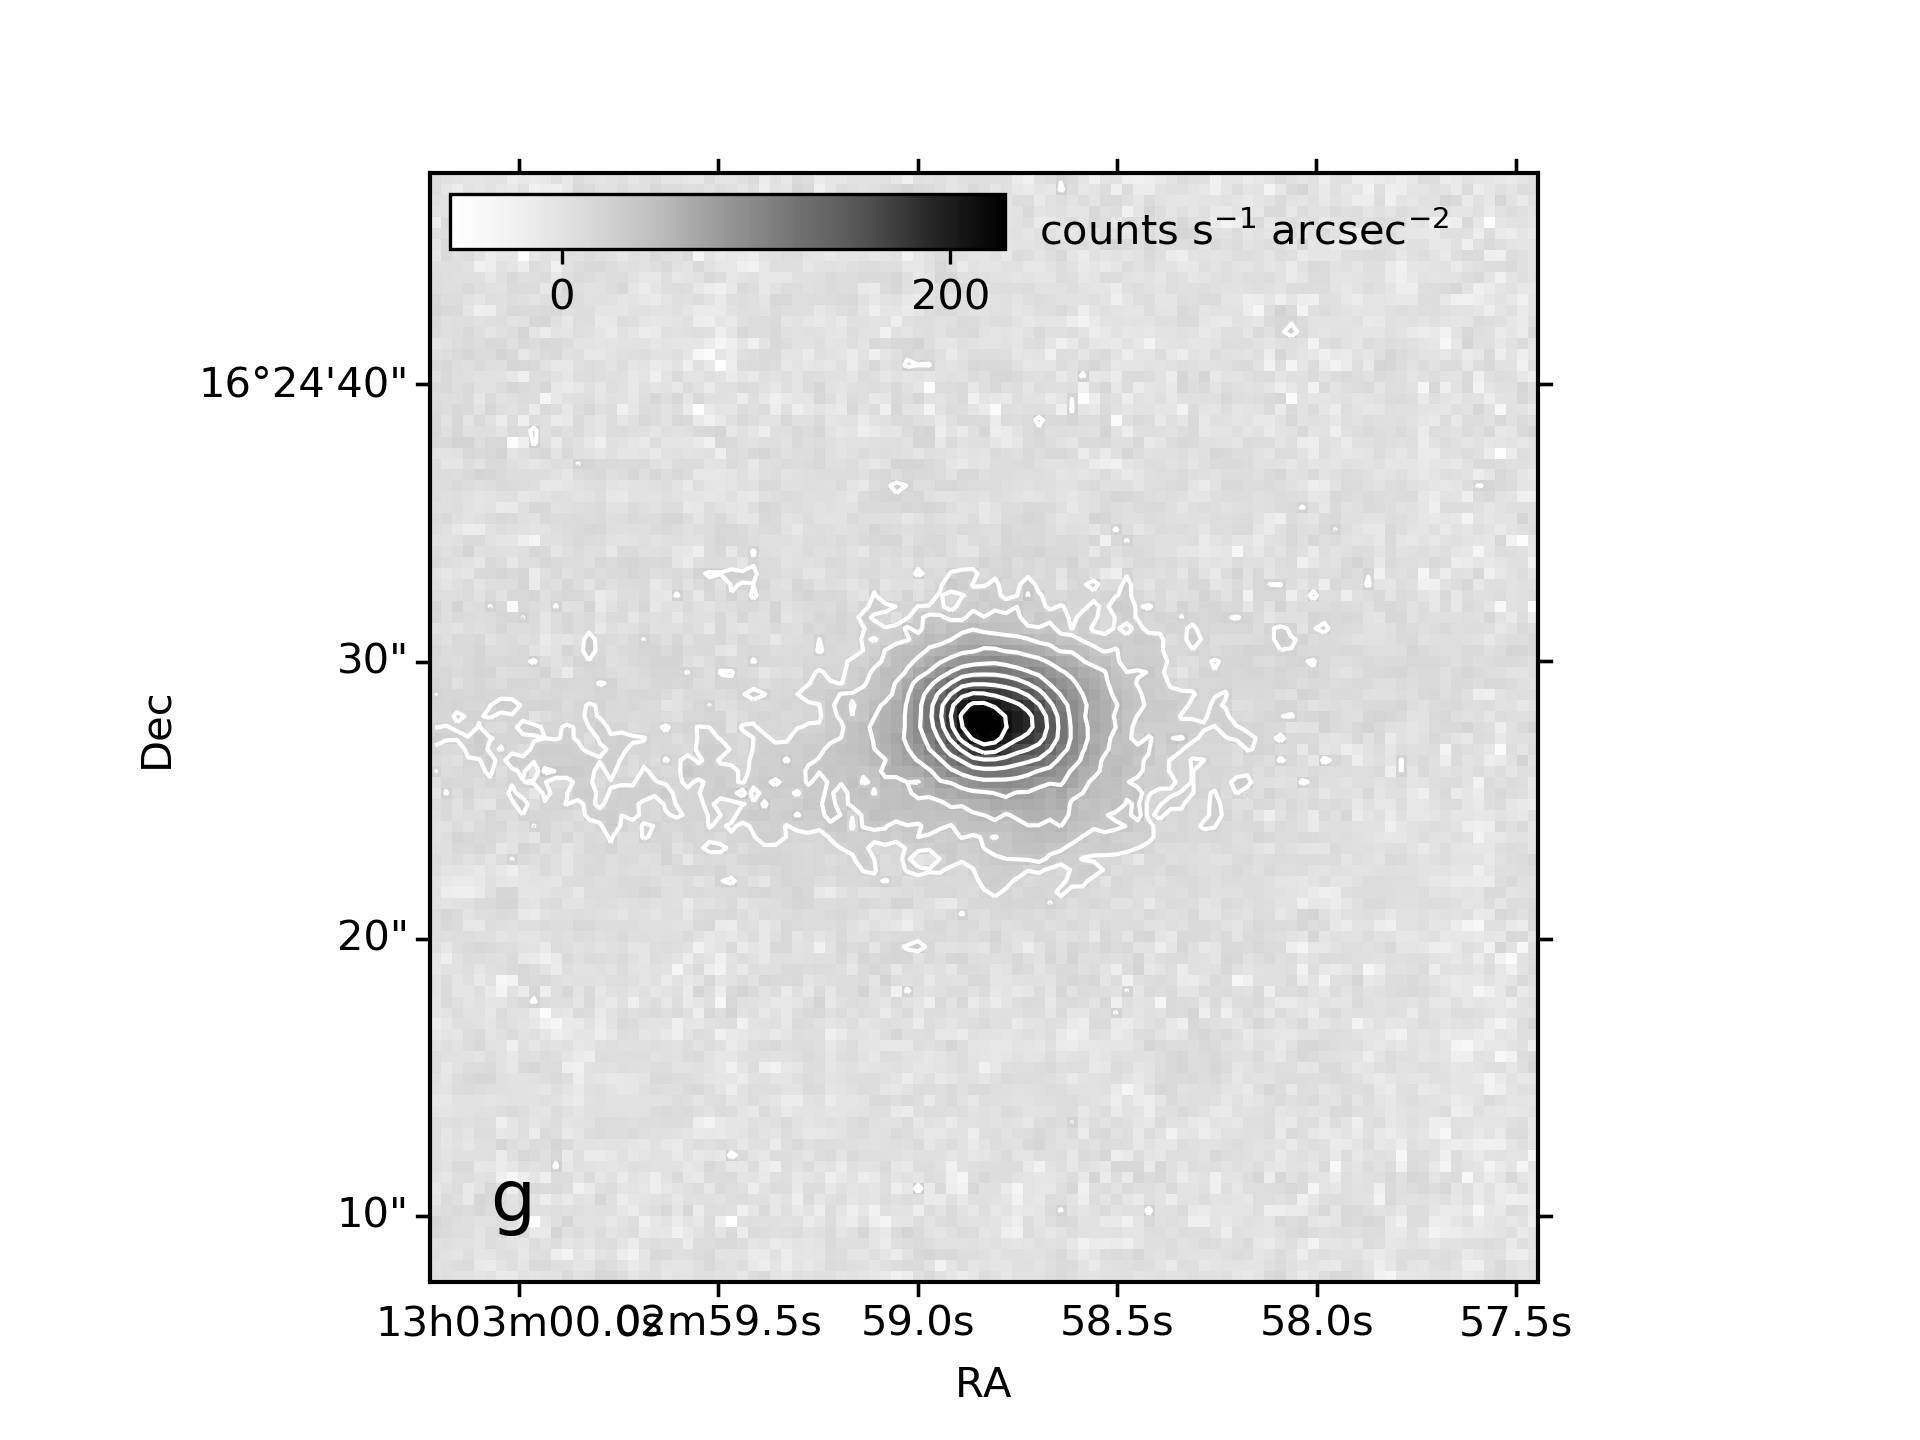
\includegraphics[width=0.6\textwidth]{images/paper3/contours_g.jpg} \\
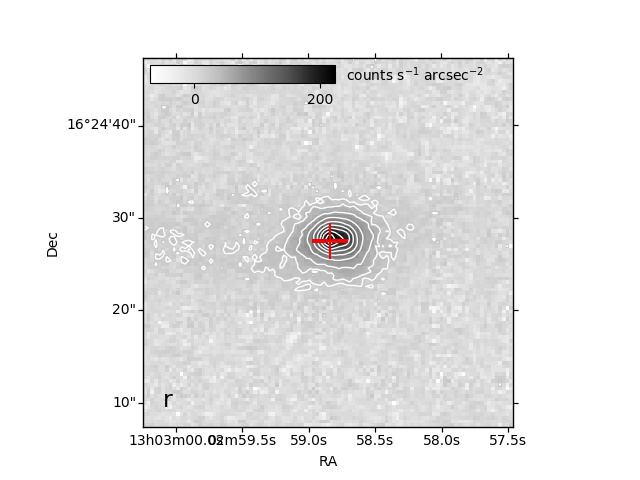
\includegraphics[width=0.6\textwidth]{images/paper3/contours_r.jpg} \\
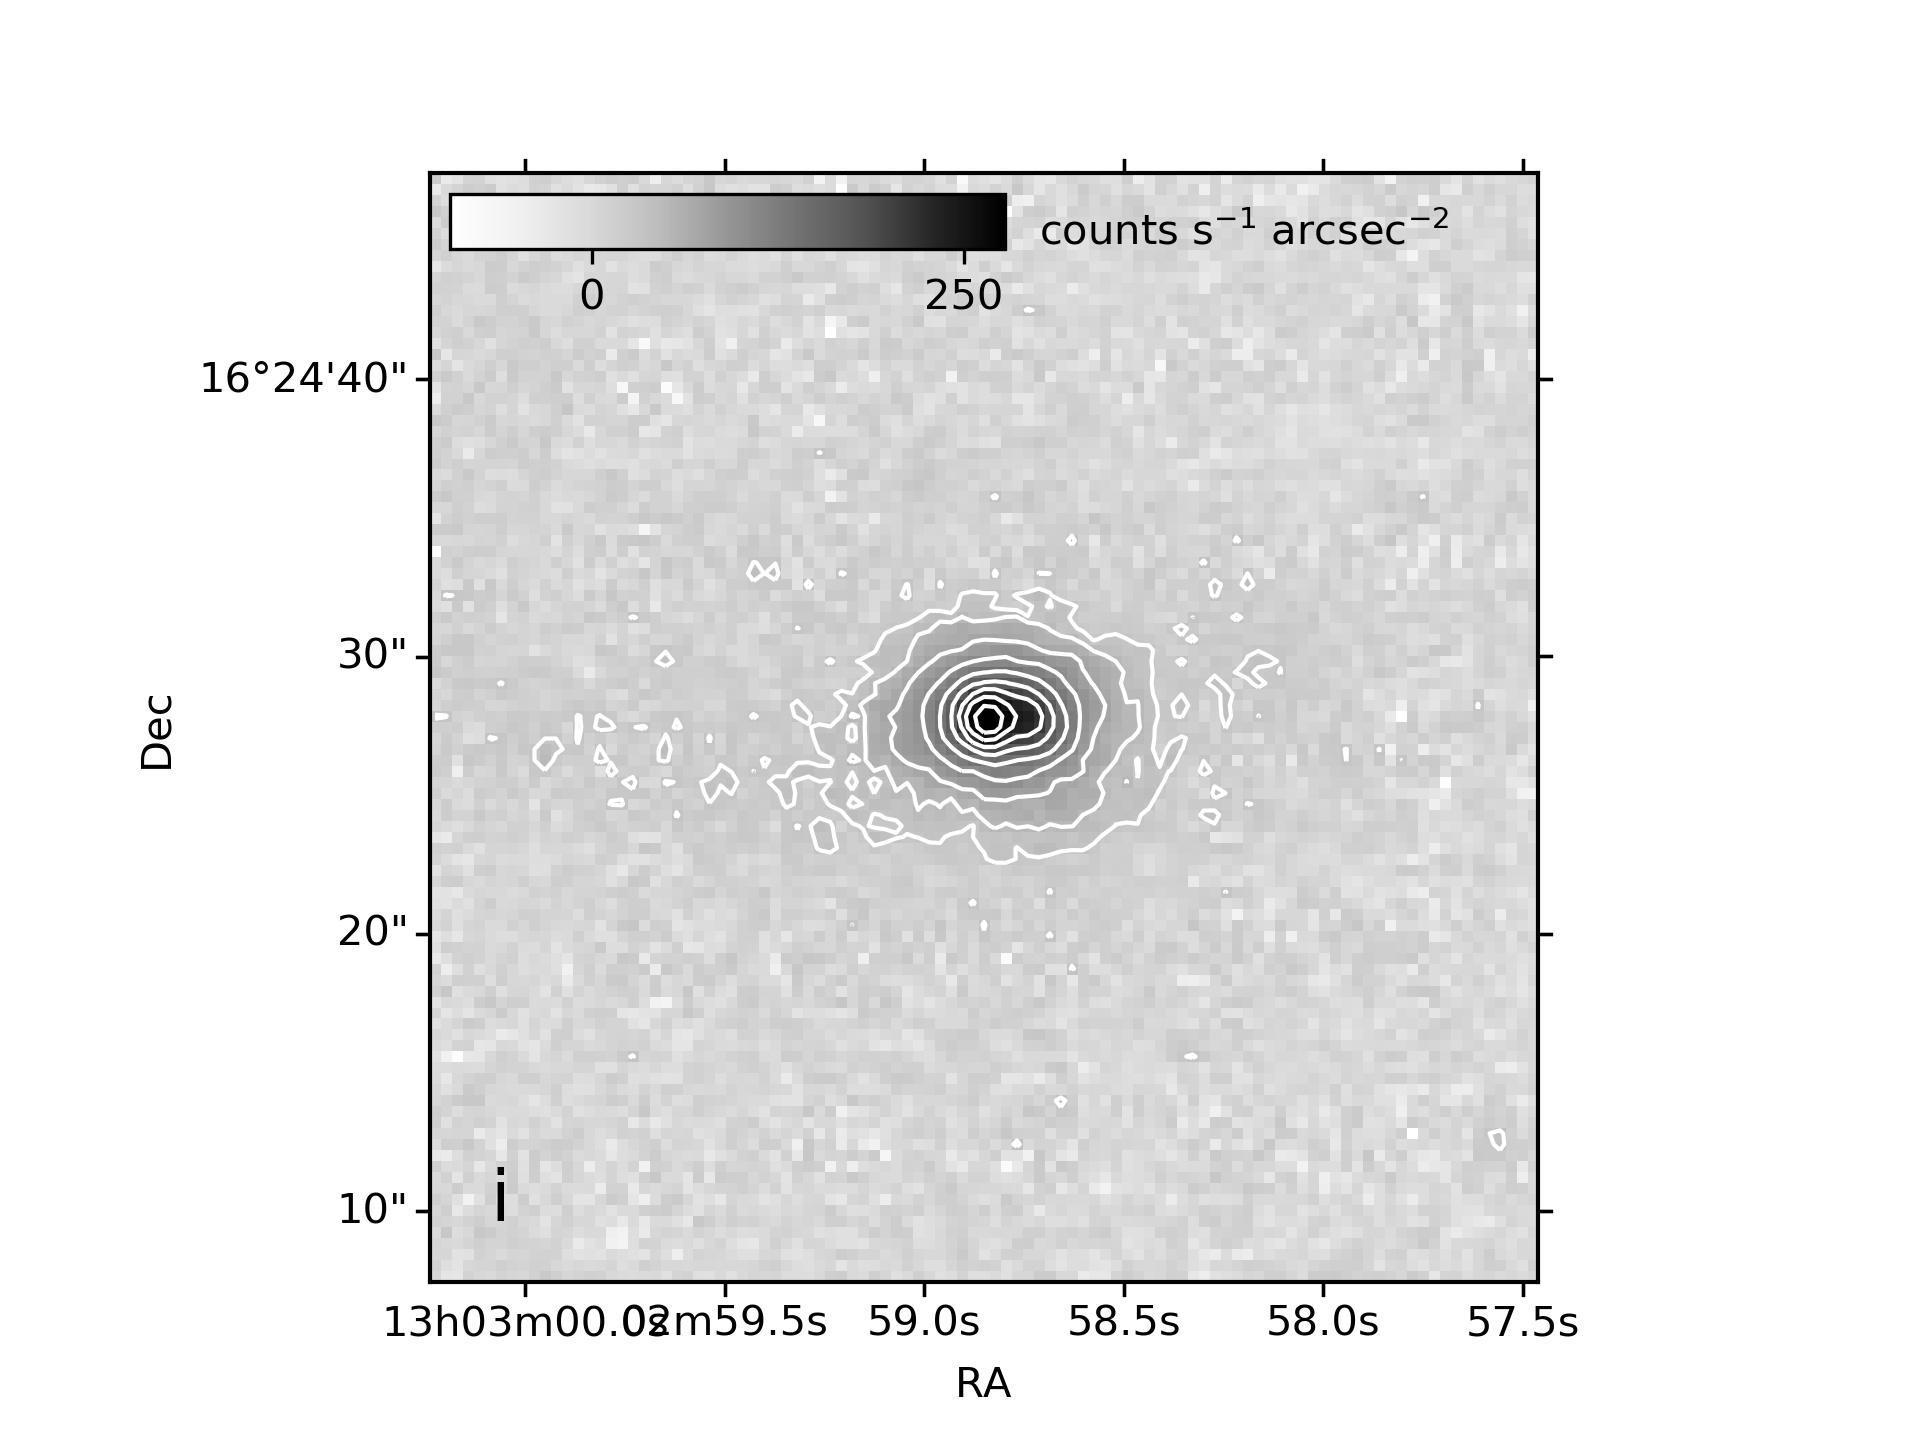
\includegraphics[width=0.6\textwidth]{images/paper3/contours_i.jpg}
\caption[]{\textbf{Left:} SDSS \emph{g}-band image of Mrk 783. \textbf{Center:} SDSS \emph{r}-band image of Mrk 783. \textbf{Center:} SDSS \emph{i}-band image of Mrk 783. Each image is in units of specific intensity ($\si{counts.cm^{-2}.s^{-1}}$). The contours are defined as $3(2^n)\sigma_{sky}$, where $\sigma_{sky}$ is the RMS of the background and $n\ge 0$. }
\label{fig:contours}
\end{figure}

The galaxy has been classified as a lenticular galaxy by \citep{Petrosian07}.
However, a quick look analysis of the SDSS images (e.g. Fig.\,\ref{fig:rgb_sdss}) revealed the presence of a faint extended structure on the east side of the nucleus, possibly a spiral arm or a tidal tail.
Fig.\ref{fig:contours} shows the \emph{g}, \emph{r} and \emph{i}-band images of Mrk 783 in units of surface intensity ($\si{counts.cm^{-2}.s^{-1}}$).
Superimposed on the images there are contours of iso-intensity which starts from $3\sigma_{sky}$, where $\sigma_{sky}$ is the RMS of the background.
The images show that the faint structure observed in the RGB image is real, even thought is barely over the $3\sigma$ detection limit.


%\textbf{non sono sicuro che questa sezione sia utile. La lascio ma non adatto il resto per ora.}

%To have a better insight on the morphology of the galaxy I produced a surface brightness profile.
%I measured the instrumental surface brightness with IRAF task \verb!ellipse! and then I calibrated the data with the calibration constants present in the SDSS file header.
%Then, I tried to fit the resulting profile with a typical profile of the nucleus of early type galaxies, the deVaucouleurs profile:
%\begin{equation}
%    \label{eq:devauc}
%    \mu_{deV} = \mu_e + 8.325\left[\left(\frac{R}{R_e}\right)^{1/4}-1\right],
%\end{equation}
%where $\mu_{e}$ is the surface brightness at the effective radius (the radius at of the isophote containing half the luminosity of the galaxy), $R_e$ is the effective radius and $R$ is the distance from the nucleus that I assumed being the AGN.
%Fig.\,\ref{fig:mrk_dev} shows the brightness profile and the relative best fitting deVaucouleurs profile.
%The profile fits relatively well only in the central part.
%At low radii it is possible to observe the flattening of the curve caused by the seeing, while at large radii the measured profile is brighter than the theoretical one which can be interpreted as a sign of the presence of a disk, in agreement with \citet{Petrosian07} classification.

%\begin{figure}
%\centering
%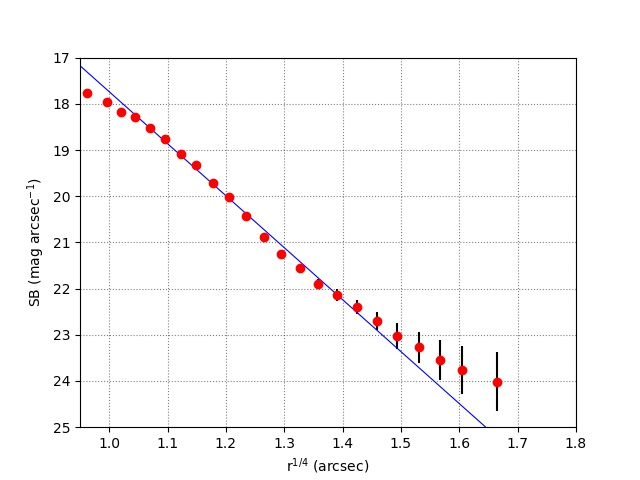
\includegraphics[width=0.7\textwidth]{images/paper3/devoc.jpg} 
%\caption[]{\emph{g}-band surface brightness profile of Mrk 783. The red dots are the data. The blue line is the best fitting de Vaucouleurs profile.} 
%\label{fig:mrk_dev}
%\end{figure} 

Fig.\,\ref{fig:contours} also shows that there seems to be a light excess $\sim 1\,\si{arcsec}$ west of the AGN, in the position corresponding to the second continuum observed in Fig.\,\ref{fig:three_spectra} and \ref{fig:flux_distr}.
This excess become more prominent moving towards redder wavelengths, i.e. the shape of the contours deviate from an ellipse more in the \emph{r} and \emph{i} images than in the \emph{g} image.

Fig.\,\ref{fig:mrk_gr} shows a $g-r$ image of the galaxy.
The AGN has a blue color ($g-r \simeq -1$) while the other structure has a red color ($g-r\simeq 1$), confirming that the secondary structure is redder than the AGN.
A $g-r$ color $\simeq 1$ is typical of stars with a temperature between $4000$ and $5000\,\si{K}$ i.e. K type stars \citep{Fukugita11}.
It is, therefore, possible that this light excess might be originated by an over-concentration of K stars.
The images has not been corrected for Milky Way extinction, but according to the calibration of \citet{Schlafly11} it is of the order of $0.09\,\si{mag}$ in the \emph{g}-band and $0.07\,\si{mag}$ in \emph{r}-band, therefore it will not particularly influence these results.

\begin{figure}
\centering
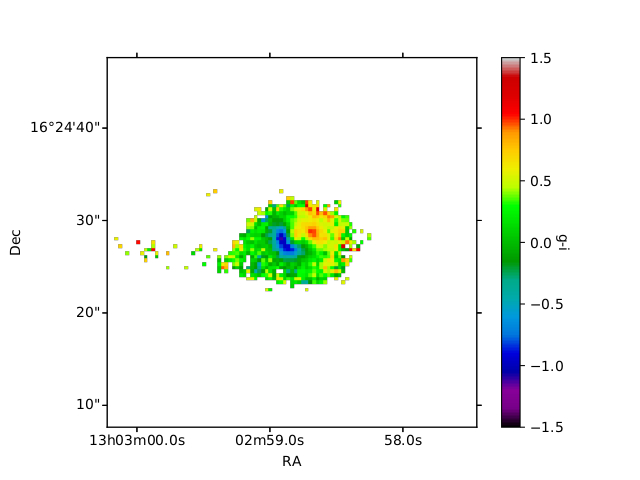
\includegraphics[width=0.7\textwidth]{images/paper3/mrk783color.jpg} 
\caption[]{$g-r$ image of Mrk 783. It is possible to see how the galaxy is sharply divided in two regions. On the left, the AGN has a negative color while the second pointlike structure has a positive color. The difference in color between the two sides is $\sim 2\,\si{mag}$.} 
\label{fig:mrk_gr}
\end{figure} 

The origin of this concentration is puzzling.
A possibility is that this structure is the nucleus of a galaxy that merged with Mrk 783. 
In this scenario, the faint extended structure on the east side of the nucleus, would be a tidal tail produced by the interaction.
This will also explain the presence of a single extended structure.
If the extended structure were a spiral arm, there should have been another similar arm on the other side of the galaxy, since the minimum number of spiral arms in a galaxy is $2$ \citep{Donghia15}.
However, also the opposite situation is possible, where the stellar structure is the real nucleus of Mrk 783 and the AGN has been accreted as a result of the interaction.

Another possible scenario is that the supermassive black hole was kicked out of the galaxy nucleus during a merging episode.
These events are rare but not impossible since such scenario have been predicted by numerical simulations and some candidates have already been discovered \citep[for a review see][]{Komossa12}.
Considering the possibility of a merging event as a possible origin of the secondary structure, it should be noticed that the merging  might have also been the trigger of the AGN activity \citep{Hong15}.

An alternative possibility is that the stellar structure is a star forming region.
In this case the red color of this region might be due to dust extinction, more than by the presence of old stars.
The presence of star formation in Mrk 783 is strongly suggested by the red WISE color $W3-W4=2.6$ and by the spectral energy distribution (SED) of the galaxy (Fig.\,\ref{fig:SED_mrk}).
The SED has been fitted with an AGN template from \citet{Polletta07} (the BQSO template in particular) and of a star forming galaxy (M 82).
FIRST and NVSS data, together with \citet{Congiu17} measurements has been used to constraint the synchrotron emission.
The main result of the analysis is that the infrared region of the SED seems to be dominated by star formation.
The estimated star formation rate is of $\sim 10-20\,\si{M_{\odot}.yr^{-1}}$.

\begin{figure}
\centering
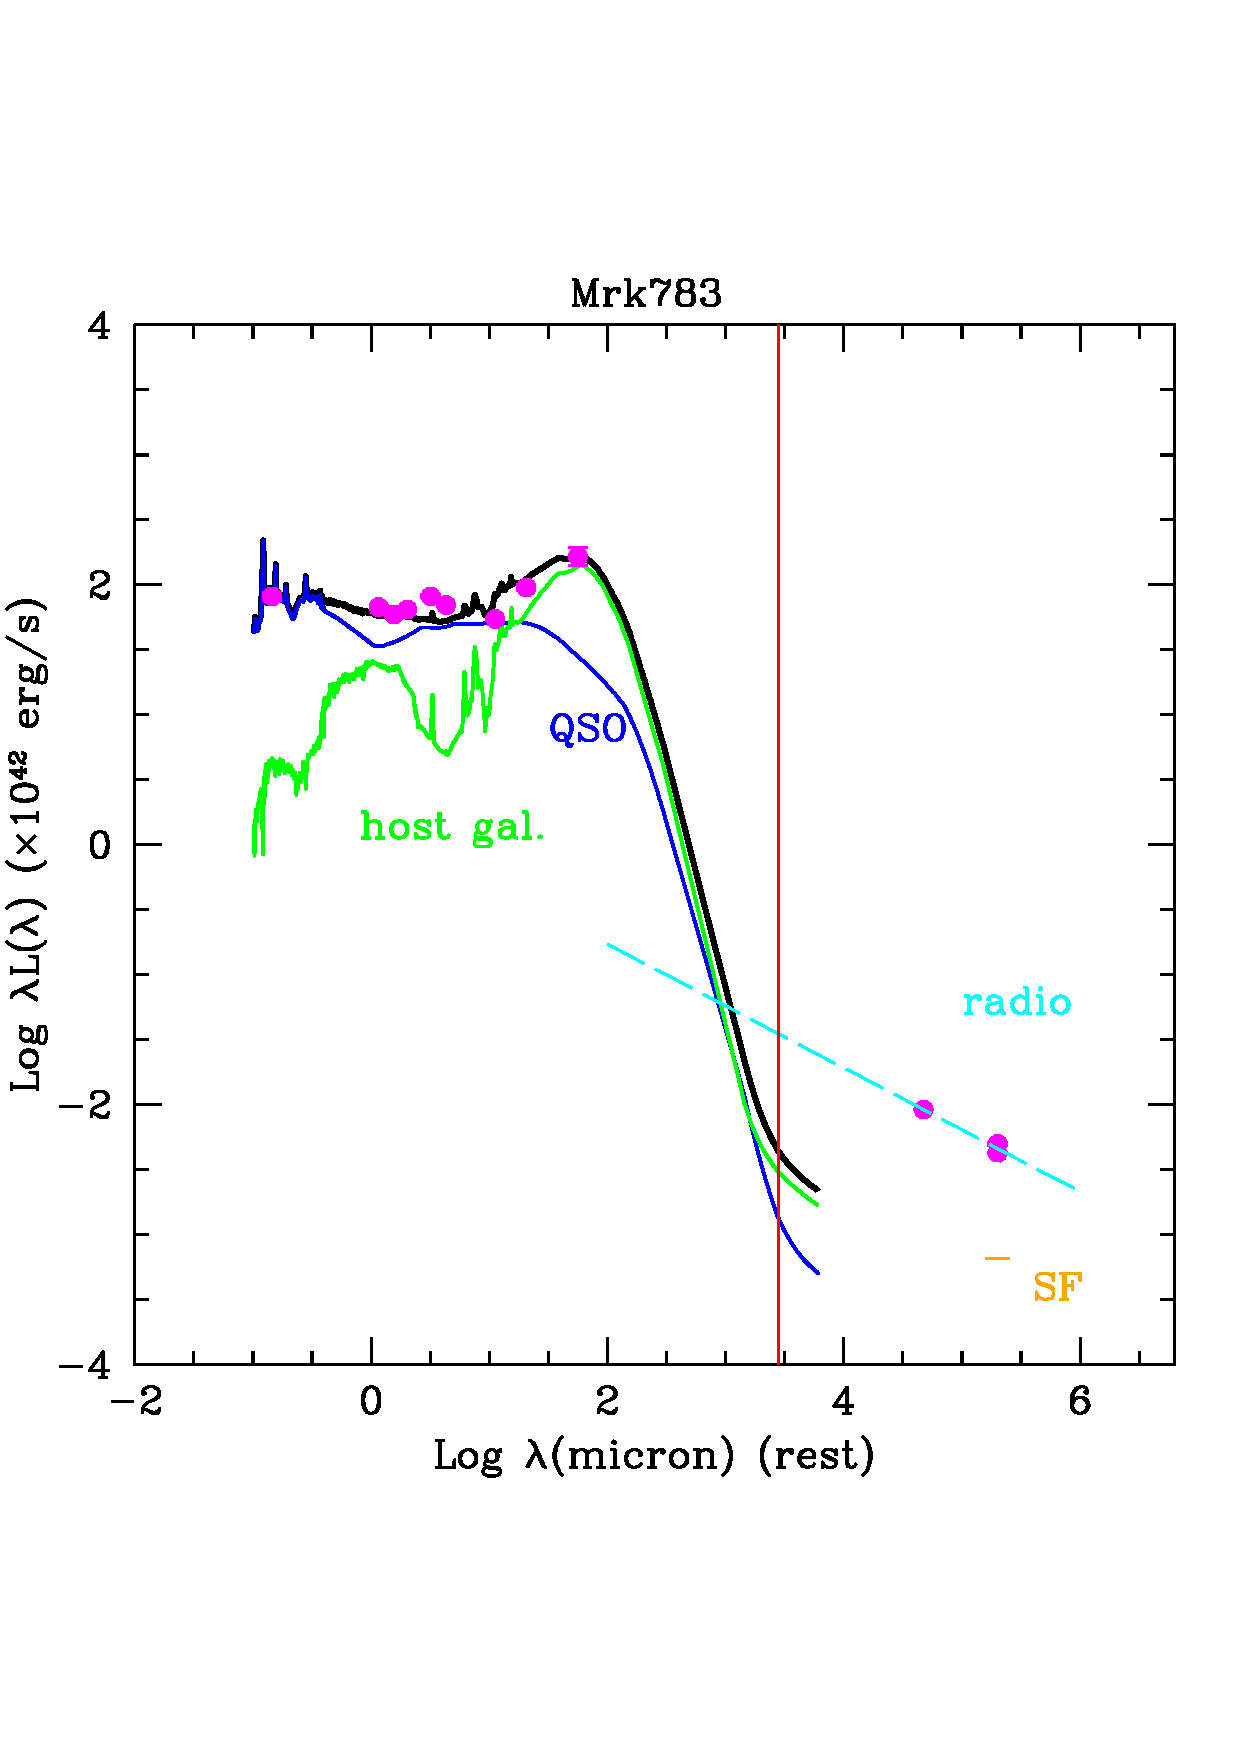
\includegraphics[width=0.7\textwidth]{images/paper3/mrk783_senza_UVOT.pdf} 
\caption[]{SED of Mrk 783 in the visible, infrared and radio band. The flux measurements have been recovered from the NED, with the exception of the $5\,\si{GHz}$ flux that comes from \citet{Congiu17}. The solid line represent the best fitting model, composed by an AGN template (BQSO template from \cite{polletta07} with $A(V)=0.3$, in blue) and a starburst template (M 82, in green).
The cyan dashed line is the power-law contribution of the jet.} 
\label{fig:SED_mrk}
\end{figure} 

To discern between these scenarios is not an easy task.
A detailed analysis of the kinematics of the central regions of the galaxy might reveal where is located its center of mass.
In such a way it will be possible to understand which one between the AGN and the secondary structure\footnote{For the sake of simplicity I will call this structure the secondary nucleus from now on.} is the real nucleus of the galaxy.
The kinematics might also reveal if one of the two structure has been accreted in a merging event or if they both belongs to the galaxy.
In the first case the kinematic of the accreted structure should be disturbed wit respect to the kinematics of the host galaxy itself, while in the second case there should not be any difference.

\subsection{Environment}
\label{sec:environment}

In the previous section I discussed how the galaxy might have been merged with a companion.
However, the probability of a merging event is higher if the merging galaxies are located in a group composed by multiple objects \citep{Kampczyk13}.
For this reason I decided to investigate the vicinity of Mrk 783 to look for other objects that might be gravitationally connected to the target.

Mrk 783 seems quite isolated but there is at least one galaxy, J1302+1625 (source A in Fig.\,\ref{fig:finding_chart}), that might be close enough. 
No redshift measurement is available for this object and for this reason the TNG spectrum has been acquired.
During this observation the slit was positioned in order to observe also J1303+1624 (source B in Fig.\,\ref{fig:finding_chart}) since it was close enough to the slit during the LDSS-3 observations to be related to the extended emission observed in panel a) and b) of Fig.\,\ref{fig:three_spectra} (see Sec.\,\ref{sec:2dspectra}).

The distance of source J1302+1625 and J1303+1624 from the nucleus of Mrk 783 are $\sim 73\,\si{arcsec}$ and $\sim 32\,\si{arcsec}$ respectively, corresponding to a projected distance of $\sim100$ and $\sim42\,\si{kpc}$ at Mrk 783 redshift.
Therefore, if their redshift is similar to that of Mrk 783 they would be close enough to be gravitationally connected.
Unfortunately, as it has been mentioned in Sec.\,\ref{sec:obs_spec}, the absolute wavelength calibration of the TNG spectrum is not reliable.
However, part of the extended emission of Mrk 783 fell inside the slit during the observation and its spectrum can be used as a reference to estimate the redshift of the two sources (Fig.\,\ref{fig:finding_chart}).

Both J1302+1625 and J1303+1624 has been detected.
J1302+1625 spectrum shows a continuum emission and some emission lines ([\ion{O}{III}]$\lambda4959$, [\ion{O}{III}]$\lambda5007$, $\Ha$).
This is in agreement with the disk-like morphology observed in SDSS and AFOSC images.
On the other hand, J1303+1624 shows a faint featureless continuum, in agreement with SDSS classification of the object as a star.
Moreover, since the lines produced in Mrk 783 ENLR are clearly detected, if J1303+1624 were the origin of the most extended emission in panel a) and b) of Fig.\,\ref{fig:three_spectra} lines should have been detected also in this spectrum.
This confirms that all the extended emission observed in Fig.\,\ref{fig:three_spectra} belongs to Mrk 783.

\begin{figure}
\centering
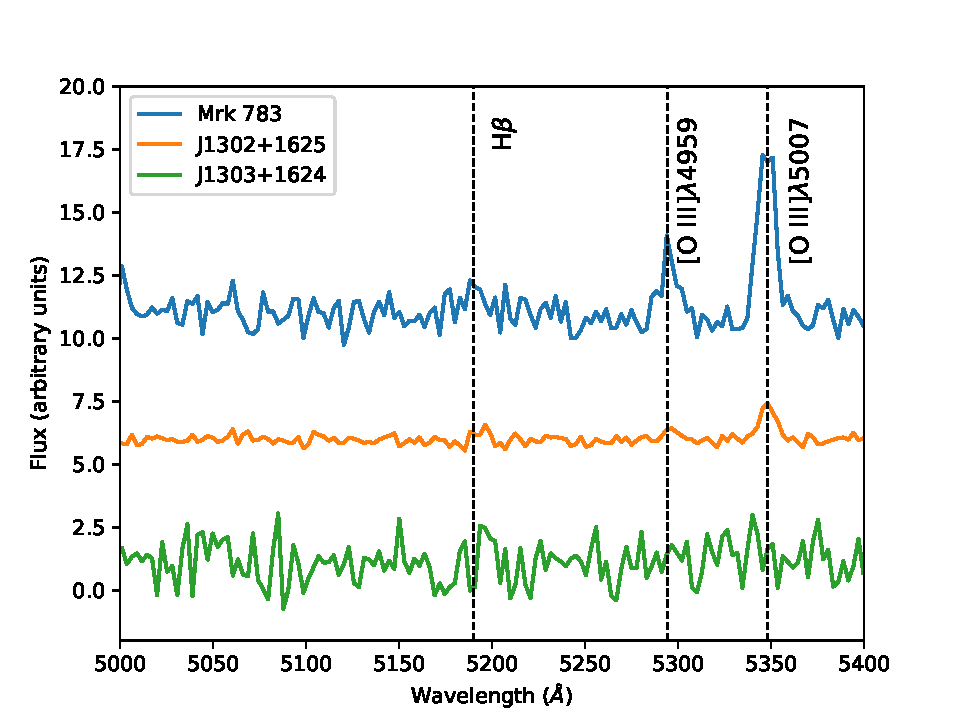
\includegraphics[width=0.7\textwidth]{images/paper3/companions_spec.pdf} 
\caption[]{$\Hb$ region of the TNG spectra. In blue is shown the spectrum of Mrk 783, in orange the spectrum of J1302+1625 and in green the spectrum of J1303+1624. The vertical dashed lines show the position of the principal emission lines observed in this wavelength range. I assumed as a reference the position of Mrk 783 lines. All the spectra have been normalized at $5100\,\si{\angstrom}$ and the blue and orange spectra have been shifted for the sake of clarity.
It is possible to see that the emission lines of Mrk 783 and source A are well aligned, while source B does not show any feature in this wavelength range.} 
\label{fig:companions_spec}
\end{figure} 

Fig.\,\ref{fig:companions_spec} shows the spectra of the three object.
They all have been normalized at $5100\,\si{\angstrom}$.
Mrk 783 and J1302+1625 show the same emission lines at the same position. 
To have a precise measurement of the wavelength of the [\ion{O}{III}]$\lambda5007$ line I fitted it in each object with a Gaussian function, using a Monte Carlo algorithm to evaluate the error on the position.
The result is that the line in Mrk 783  is at $5347.6\pm0.4\,\si{\angstrom}$ while in J1302+1625 is at $5348.3\pm0.4\,\si{\angstrom}$.
The difference between the two wavelength of the two line is $\sim 0.7\,\si{\angstrom}$ ($\sim 50\,\si{\kms}$).
This confirms that the vicinity of the two object is not just a projection effect.
Tab.\,\ref{tab:companions} shows the main properties of J1302+1625 and J1303+1624.

The observation of another galaxy at a distance of $100\,\si{kpc}$ from Mrk 783 confirms that the object is part of a (small) group of galaxies.
Actually the two objects are close enough that they might already interacting, even though the undisturbed morphology of J1302+1625 suggests that the interaction is still in the early phases.

Since the probability of merging are higher in groups \citep{Kampczyk13} the scenario described above where the properties of Mrk 783 are the result of a merging event is even more plausible now, even though a final confirmation will require better data and a more detailed analysis.

\begin{table}
    \centering
    \caption{Main properties of the companion sources of Mrk 783.}
    \label{tab:companions}
    \begin{threeparttable}
    \begin{tabular}{lcccccc}
    \hline
    \hline
    Source& Name & Type& RA & Dec & \emph{g}& Distance\\
          &      &     & (hh:mm:ss)&(dd:mm:ss)& (mag) &($\si{arcsec}$)\\
    \hline
    A &J1302+1625&Galaxy &$13$:$02$:$57.20$&$+16$:$25$:$37.1$&$18.7$&$72.7$\\
    B &J1303+1624&Star &$13$:$03$:$00.42$&$+16$:$24$:$04.3$&$21.70$&$32.3$\\
    \hline
    \end{tabular}
    \begin{tablenotes}
    \item From left to right: (1) Source name in Fig.\,\ref{fig:finding_chart}, (2) name of the source, (3) SDSS classification of the source, (4) right ascension, (5) declination, (6) \emph{g}-band magnitude measured from AFOSC image, (7) distance in arcsecond from the AGN, (8) redshift measured from TNG spectrum.
    \end{tablenotes}
    \end{threeparttable}
\end{table}


\section{Spectral Analysis}
\label{sec:spectral_anal}

\subsection{Spectra Extraction and Line Fitting}
\label{sec:extraction}
To better analyze the properties of the LDSS-3 spectra as a function of the distance from the AGN, I divided each two-dimensional spectra in $1\,\si{arcsec}$ bins and I extracted one-dimensional spectra from each one of them showing emission lines.
All the spectra have been corrected for galactic extinction using the standard CCM extinction law \citep{Cardelli89}, with $R = 3.1$ and the absorption in the $V$ band $A(V)$ provided by the NASA/IPAC Extragalactic Database\footnote{https://ned.ipac.caltech.edu/} (NED) and extracted from \citet{Schlafly11}.
A correction for telluric absorption has also been applied, since $\Ha$ falls close to one of the major telluric absorption.

An accurate measurements of the emission line flux, especially for the Balmer lines, usually requires a subtraction of the underlying stellar continuum, since stellar absorption might significantly contribute to the line flux.
This process is not needed in the nucleus of type 1 AGN, since the AGN continuum dominates over the stellar continuum and the influence of stellar absorption is negligible.
On the other hand, outside the nucleus the stellar emission is the dominant continuum source and an accurate subtraction should be performed.

However, to obtain reliable results this procedure must be performed on high signal to noise ratio (SNR) spectra.
Since the signal-to-noise ratio of the continuum is low in most of the bin extracted from the LDSS-3 spectra uncontamined by the AGN, I decided to not perform the stellar continuum subtraction.

After the extinction correction I measured the flux of the most prominent emission lines of all spectra.
I used a Monte Carlo algorithm to measure the flux, wavelength and dispersion of each emission line with errors.
Since the resolution of the instrument is relatively low ($\sim 500\,\si{\kms}$) most of the line are not resolved and they can be fitted with a single Gaussian function.
Close to the AGN, where the Balmer lines start to get broad, I used two or three Gaussian components to fit them.
In these cases, I used one Gaussian to fit the narrow component and one or two Gaussians for the broad component.

During the line fitting procedure I had to pay particular attention to the $\Ha$ and [\ion{N}{II}] doublet, since they are very close.
To obtain a better result I fitted the three lines simultaneously using one component for each line of the [\ion{N}{II}] doublet and one, two or three components for $\Ha$, according to the profile shape.
To reduce the number of free parameters I constrained the narrow components to have all the same width.
In the very nucleus of the galaxy I also had to fit the [\ion{S}{II}] doublet  simultaneously with the $\Ha$ group, because the broad components of $\Ha$ was so large to be partially blended with the doublet.
Also in this case I reduced the number of free parameters forcing the width of the narrow lines to be the same.
Fig.\,\ref{fig:pap3_deblending} shows an example of the deblending process in the nucleus of Mrk 783.

\begin{figure}
\centering
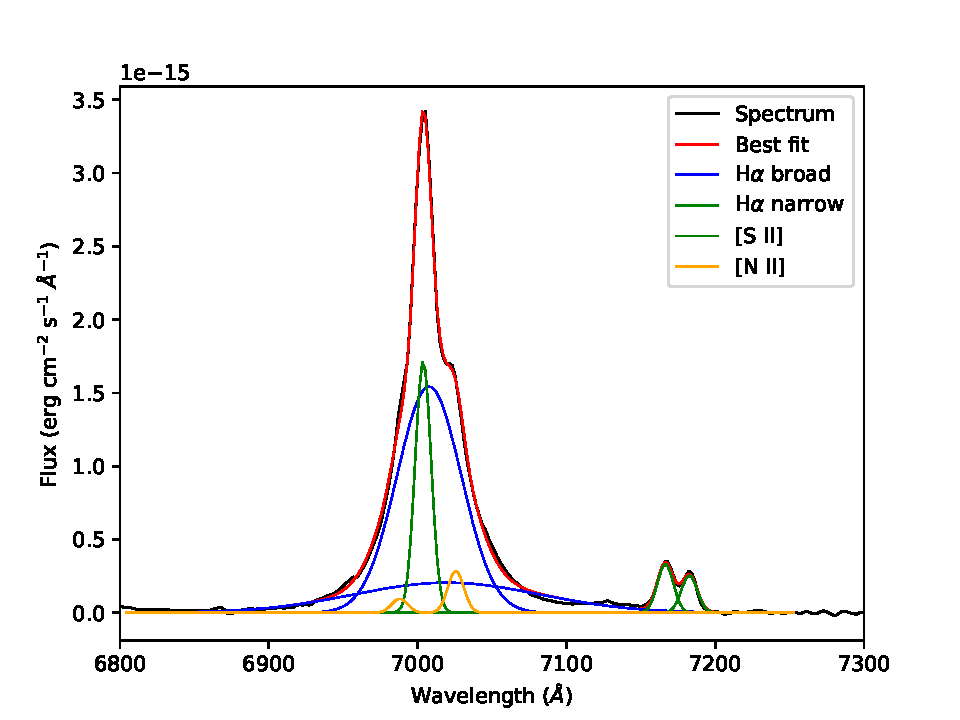
\includegraphics[width=0.7\textwidth]{images/paper3/deblending.pdf} 
\caption[]{Example of the fit of the $\Ha$ group in the nucleus of Mrk 783. In particular this is the one dimensional spectrum of the nucleus extracted from February LDSS-3 spectrum.} 
\label{fig:pap3_deblending}
\end{figure} 


\subsection{The nuclear spectrum}

\begin{figure}
\centering
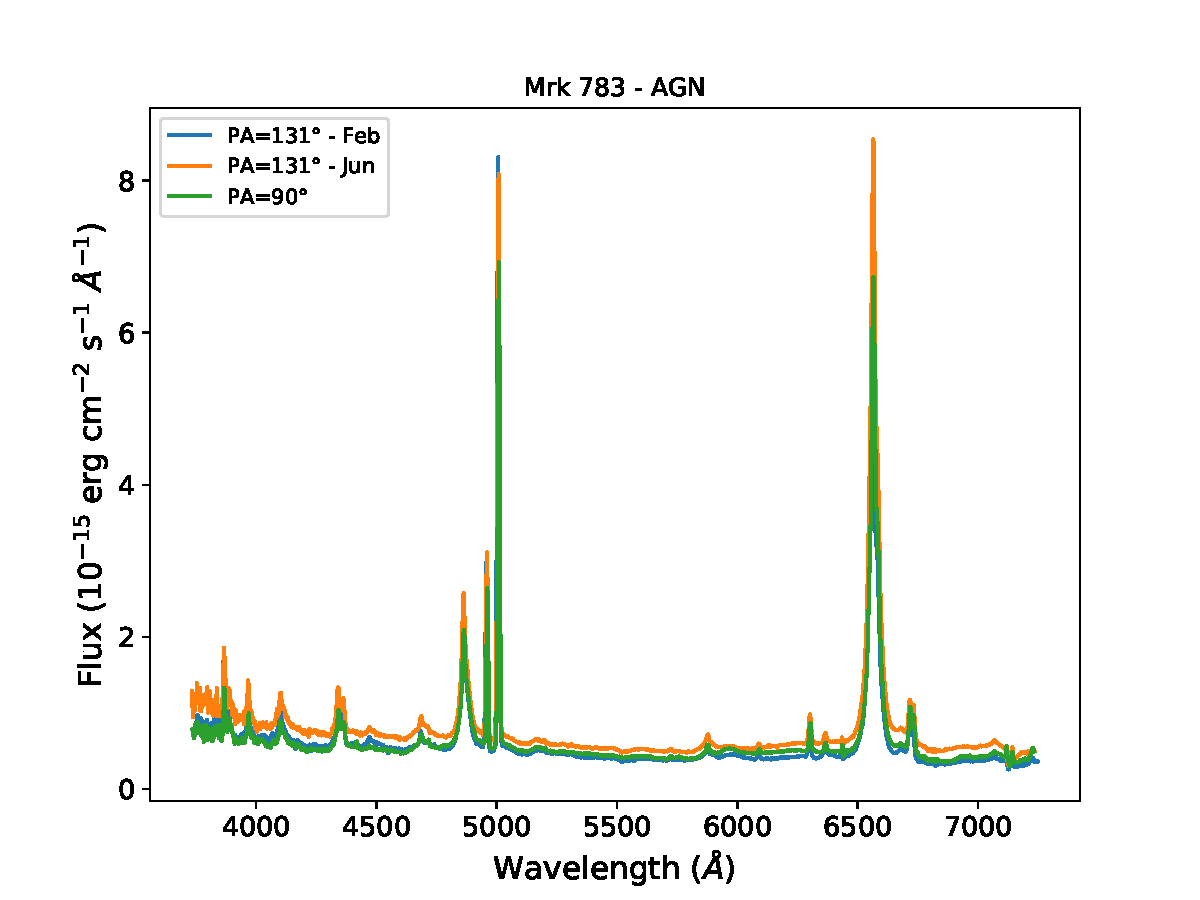
\includegraphics[width=\textwidth]{images/paper3/spectrum_nucleus.pdf} 
\caption[]{One-dimensional spectrum of the nucleus of Mrk 783 extracted from February LDSS-3 spectrum at PA $=\ang{131}$. } 
\label{fig:all_spectra}
\end{figure} 

All the three spectra of Mrk 783 acquired with the LDSS-3 spectrograph have been centered on the AGN.
There are some small differences between the three spectra, probably because of the different conditions of the sky during the observations. 
For these reasons the spectra has not been combined to produce a single spectrum of the nucleus but they will be examined separately in the following sections.
Fig.\,\ref{fig:all_spectra} shows the AGN spectrum extracted from February observation at PA $=\ang{131}$.
In this section I will consider this spectrum to check the classification of this object as a NLS1.

As stated in Sec.\,\ref{sec:pap3_intro}, the spectrum of an AGN must satisfy three requirements to be classified as a NLS1: 1) $FWHM(\Hb)<2000\,\si{\kms}$, 2) [\ion{O}{III}]$\lambda5007/\Hb<3$ \citep{Osterbrock85} and 3) Strong \ion{Fe}{II} multiplets or presence of [\ion{Fe}{VII}]$\lambda6087$ and [\ion{Fe}{X}]$\lambda6375$ lines \citep{Goodrich89}.
Mrk 783 shows a $FWHM(\Hb)\sim1500\,\si{\kms}$ and a flux [\ion{O}{III}]$\lambda5007/\Hb\sim 1.5$, that are well below \citet{Osterbrock85} limits.
On the other hand, the object shows little \ion{Fe}{II} emission (there is only some trace of the $5190\,\si{\angstrom}$ multiplet), but it shows both the [\ion{Fe}{VII}]$\lambda6087$ line and the [\ion{Fe}{X}]$\lambda6375$ (blended with the [\ion{O}{I}]$\lambda6363$ line) and other high ionization Fe lines (Fig.\,\ref{fig:fe_lines}).
Therefore the classification of Mrk 783 as a NLS1 can be confirmed.

\begin{figure}
\centering
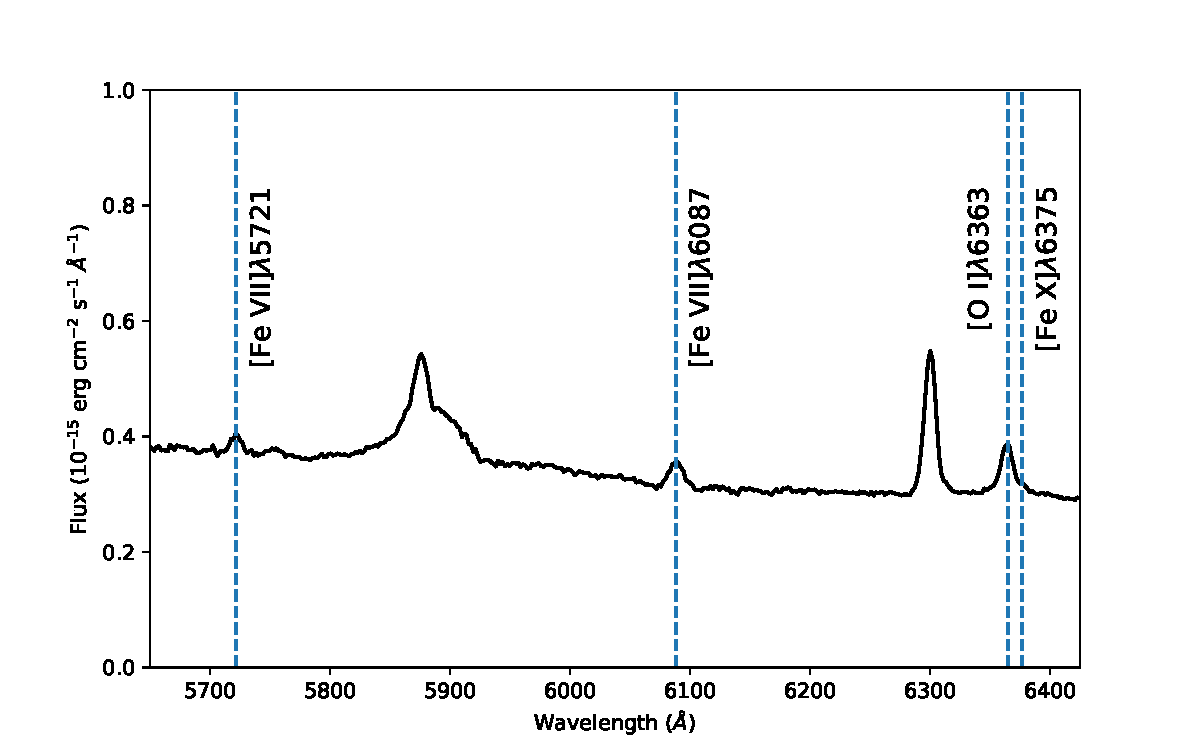
\includegraphics[width=\textwidth]{images/paper3/Fe_lines.pdf} 
\caption[]{February LDSS spectrum between $5650$ and $6425\,\si{\angstrom}$. The dashed lines show the position of [\ion{Fe}{VII}]$\lambda5721$,  [\ion{Fe}{VII}]$\lambda6087$, [\ion{Fe}{X}]$\lambda6375$,[\ion{O}{I}]$\lambda6363$.} 
\label{fig:fe_lines}
\end{figure} 

\subsection{Kinematics}
\label{sec:pap3_kinematics}

\begin{figure}
\centering
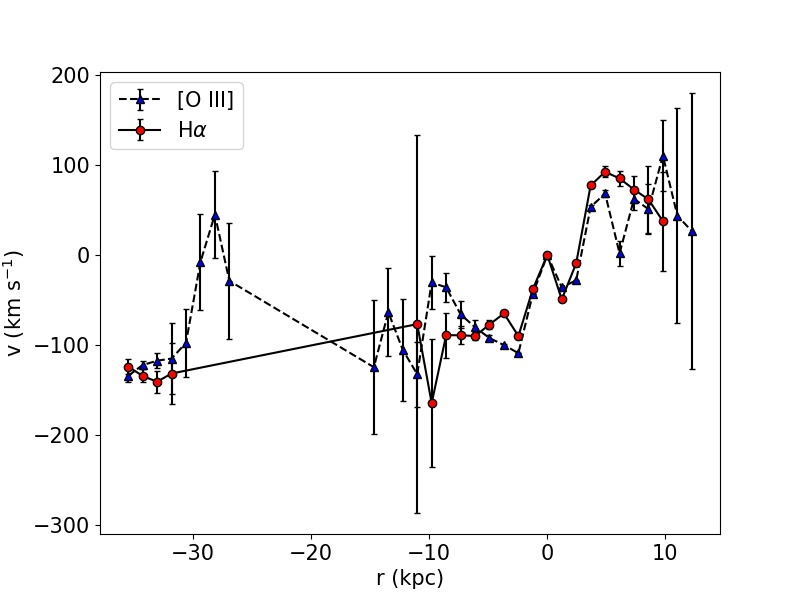
\includegraphics[width=0.6\textwidth]{images/paper3/PA131_2016_velocity.jpg}\\ 
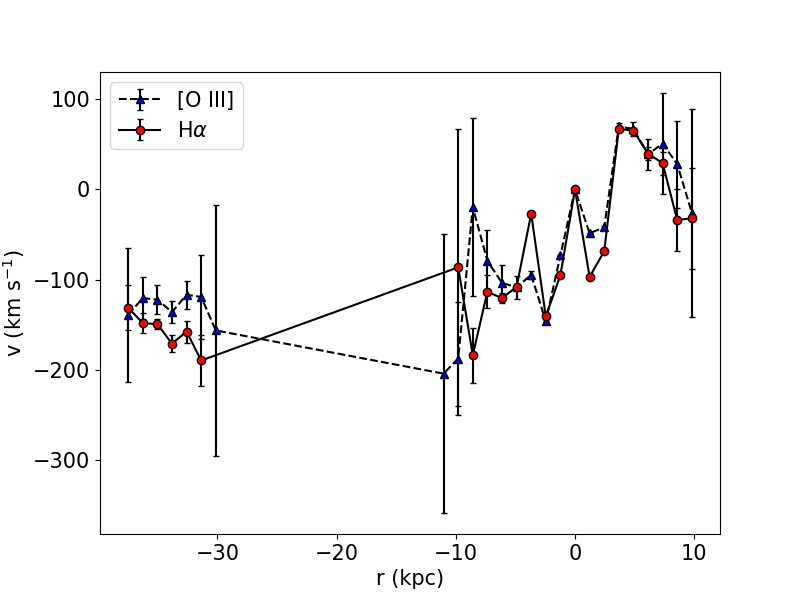
\includegraphics[width=0.6\textwidth]{images/paper3/PA131_velocity.jpg}\\ 
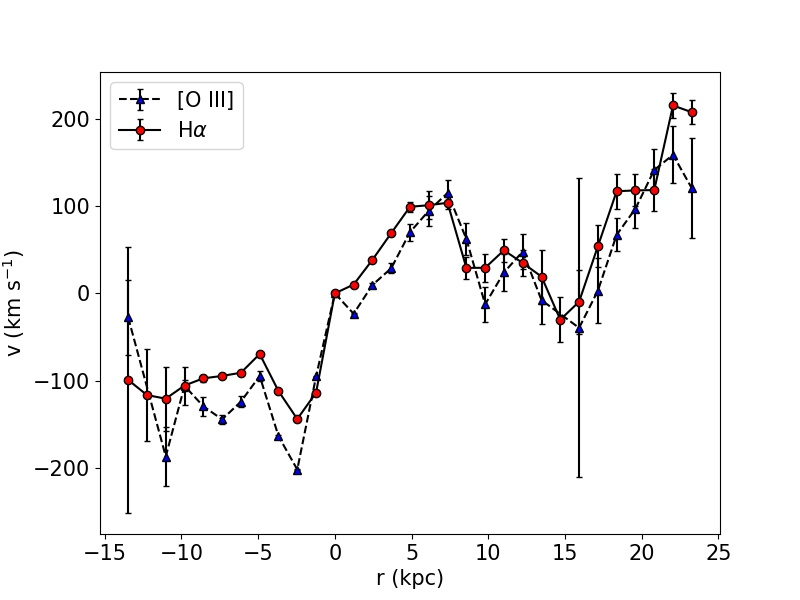
\includegraphics[width=0.6\textwidth]{images/paper3/PA90_velocity.jpg}\\ 
\caption[]{Velocity vs distance from the nucleus maps for, from top to bottom: February PA $=\ang{131}$ spectrum, June PA $=\ang{131}$ spectrum and June PA $=\ang{90}$ spectrum. Blue triangles represent [\ion{O}{III}]$\lambda5007$ velocities, the red dots are $\Ha$ velocities.
The error bars represent $1\sigma$ errors. The absence of error bars means that they are smaller than the size of the point. The velocity of the central spectrum has been considered as the systemic velocity of the galaxy.} 
\label{fig:velocity_lines}
\end{figure} 

From the position of the lines measured from the spectra I was able to produce, for each observation at each PA, a velocity vs radius plot.
In almost all the one dimensional spectra it has been possible to measure the velocity of both the narrow $\Ha$ component and [\ion{O}{III}]$\lambda5007$ and the results of the measurements are shown in Fig.\,\ref{fig:velocity_lines}.
Since the inclination of the galaxy is not known, it is not possible to correct velocities and distances, and all the values reported in this work are projected quantities.

From these plots it is possible to see that the kinematics of the gas seems significantly disturbed at all distances from the nucleus.
In particular, at PA $=\ang{90}$ the gas velocity decreases of $>100\,\si{\kms}$ between $r\simeq 7\,\si{kpc}$
and $r\simeq 15\,\si{kpc}$.
Then it starts to rise again up to velocities similar to those before the drop.
A similar feature can be observed also on the other side of the rotation curve, even though the drop and rise are significantly faster.
On the other hand, the velocity curves at PA $=\ang{131}$ are flatter with respect to the velocity curve of the other position angle, but there are faster variations.
Nevertheless, the main trend seems to indicate the presence of rotation of the gas, with a $\Delta v \simeq 200\,\si{\kms}$ at PA $=\ang{131}$ and PA $\Delta v \simeq 300\,\si{\kms}$ at PA $=\ang{90}$.
The difference of amplitude of the velocity curve is probably due to the inclination of the galaxy.
The spectrum at PA $=\ang{90}$ is probably closer to the major axis of the galaxy with respect to the spectra at PA $=\ang{131}$.

In general, the kinematics of $\Ha$ and [\ion{O}{III}]$\lambda5007$ is quite similar, most of the differences between the kinematics of the two lines are inside the error bars.
In the top and center plots is evident the absence of emission between the main body of the galaxy and the most extended region of the emission, which was already visible in Fig.\,\ref{fig:all_spectra}.

No peculiar features are observed in the position of the secondary nucleus of Sec.\,\ref{sec:morph_color}, so it is not possible to determine which one between the AGN and the secondary nucleus sits in the dynamical center of the galaxy.
Without integral field data or narrow filter images of the source to map the gas distribution, it is difficult to have a better insight on the kinematical properties of this object.

A merging event might be able to explain the disturbed kinematics.
The kinematical signature of an event of this type might be visible up to a time of $0.2-0.4\,\si{GHz}$ from the event \citep{Hung16}, therefore the merger must be relatively recent if we can still observe its effect on the gas kinematics.

Also the presence of a relativistic jet digging in the ISM might be able to influence the gas kinematics.
The radio emission discovered by \citet{Congiu17} means that a jet might have been active in this galaxy.
The structure is aligned with PA $=\ang{131}$, but there are no traces of radio emission at PA $=\ang{90}$ where the largest features are observed.
Moreover, the extension of this structure is of the order of $10\,\si{kpc}$, so it cannot be responsible for features at larger distances from the nucleus.
Therefore, if a relativistic jet has been active (or is still active) in this object it could have produced the features observed in the inner region at PA $=\ang{131}$, but it cannot be responsible for what is happening at PA $=\ang{90}$.

Up until now, the gas kinematics is, hence, another piece of evidence in support of a merging event.
If this is the correct scenario, the kinematics also helped constraining the age of the event, limiting the maximum age of the merging at $0.4\,\si{Gyr}$.


\subsection{Line ratios}
\label{sec:pap3_lineratios}

\begin{figure}
\centering
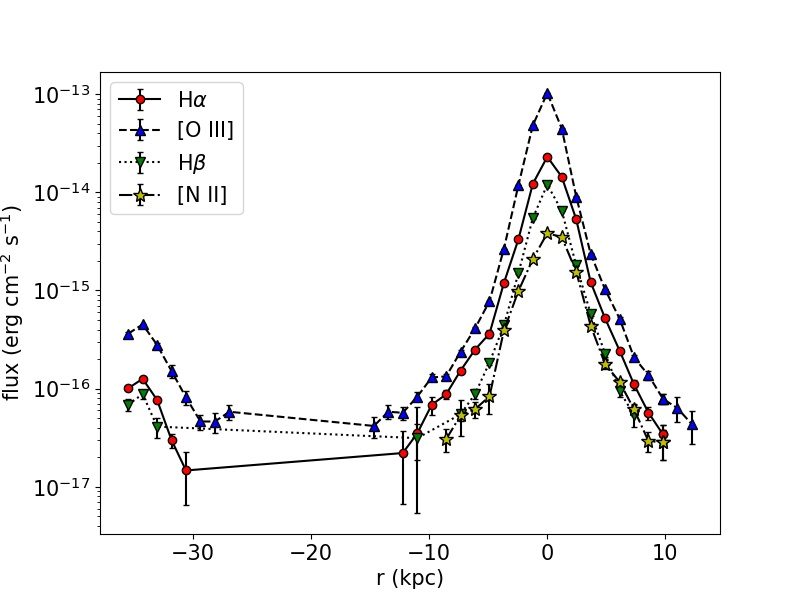
\includegraphics[width=0.6\textwidth]{images/paper3/PA131_2016_line_flux.jpg}\\ 
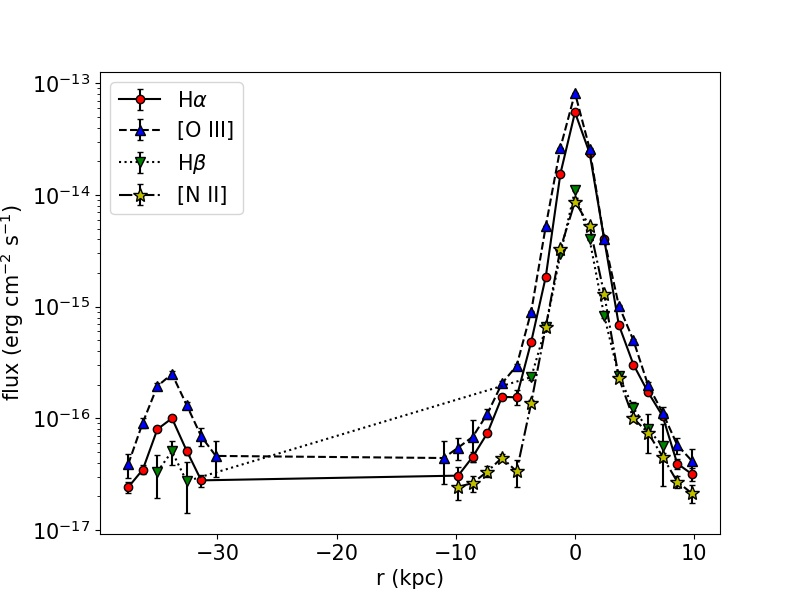
\includegraphics[width=0.6\textwidth]{images/paper3/PA131_line_flux.jpg}\\ 
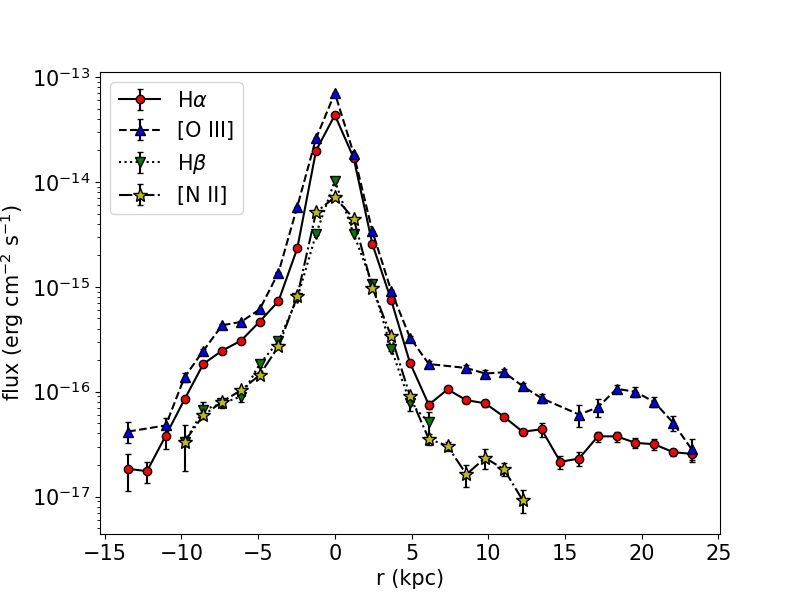
\includegraphics[width=0.6\textwidth]{images/paper3/PA90_line_flux.jpg}\\ 
\caption[]{Line flux vs distance from the nucleus plot for each LDSS-3 spectrum. From top to bottom: February PA $=\ang{131}$, June PA $=\ang{131}$ and June PA $=\ang{90}$. The error bars represent $1\sigma$ errors. Where they are not present they are smaller than the size of the corresponding point.} 
\label{fig:line_fluxes}
\end{figure} 

The extended emission has been considered, so far, the ENLR produced by the AGN.
However, in Sec.\,\ref{sec:morph_color} it has been discussed that the SED of Mrk 783 seems to have an infrared excess produced by a star formation rate of $\sim 10\,\si{M_{\odot}.yr^{-1}}$.
So, it is possible that part of the gas is ionized by young stars and not by the AGN.

To test this possibility it is possible to use the so called \emph{diagnostic diagrams}, diagrams comparing ratios between strong forbidden lines and nearby narrow Balmer lines \citep{Baldwin81,Veilleux87}.
In particular there are three different diagnostic diagrams that are used to this aim: $\log [\rm \ion{O}{III}]\lambda5007/\Hb$ vs $\log [\rm \ion{N}{II}]\lambda6584/\Ha$, $\log [\rm \ion{O}{III}]\lambda5007/\Hb$ vs $\log [\rm \ion{O}{I}]\lambda6300/\Ha$ and $\log [\rm \ion{O}{III}]\lambda5007/\Hb$ vs $\log [\rm \ion{S}{II}]\lambda\lambda6717,6731/\Ha$.

In order to better classify the emission I tried to produce all three diagrams for each spectrum.
However, while $\Ha$ and [\ion{O}{III}]$\lambda5007$ have been detected in the vast majority of the spectra, all the other lines are fainter and they are often missing.
For example, in Fig.\,\ref{fig:line_fluxes} it is possible to see the flux distribution of some of the emission lines used in the diagnostic diagrams.
Lines such as $\Hb$ and [\ion{N}{II}]$\lambda6584$ are detected only in the inner part of the galaxy.
The main consequence of this is that it will not be possible to investigate with diagnostic diagrams the ionizing source of the most extended structures.

\begin{figure}
\centering
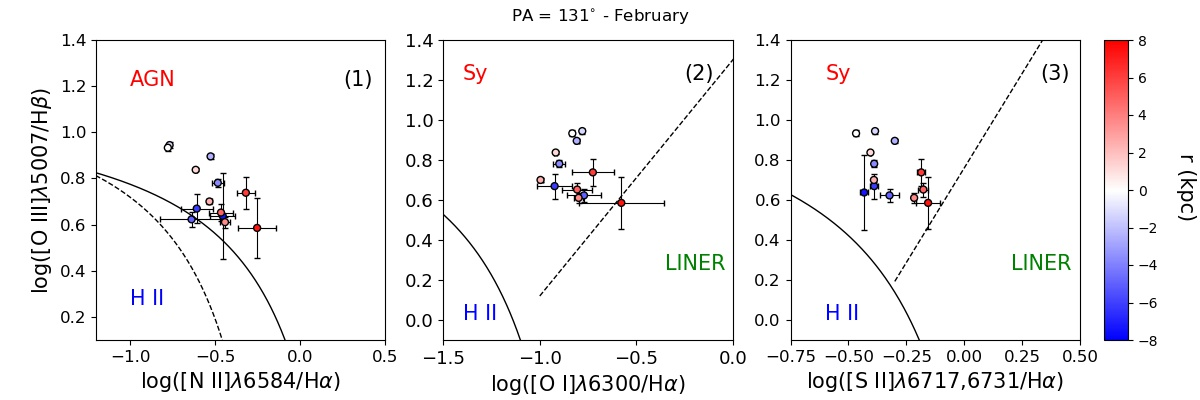
\includegraphics[width=\textwidth]{images/paper3/PA131_2016_diagnostic.jpg}\\ 
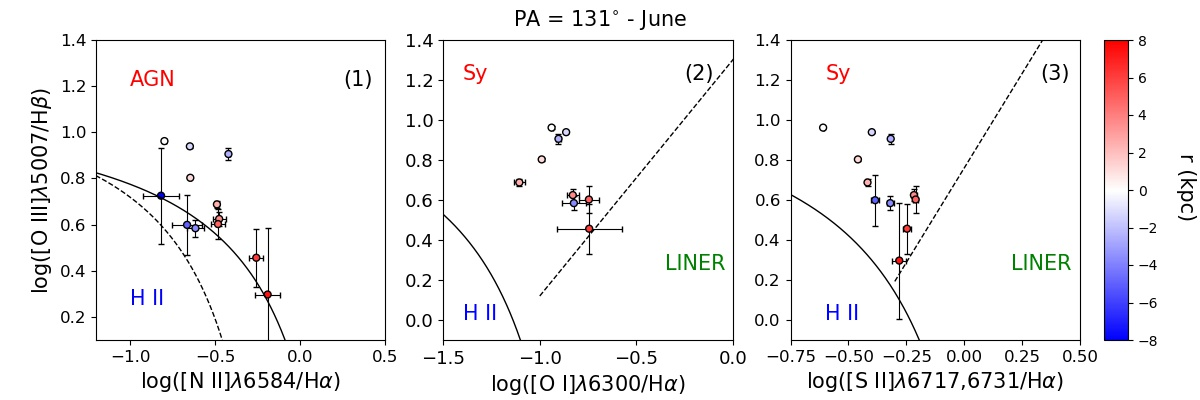
\includegraphics[width=\textwidth]{images/paper3/PA131_diagnostic.jpg}\\ 
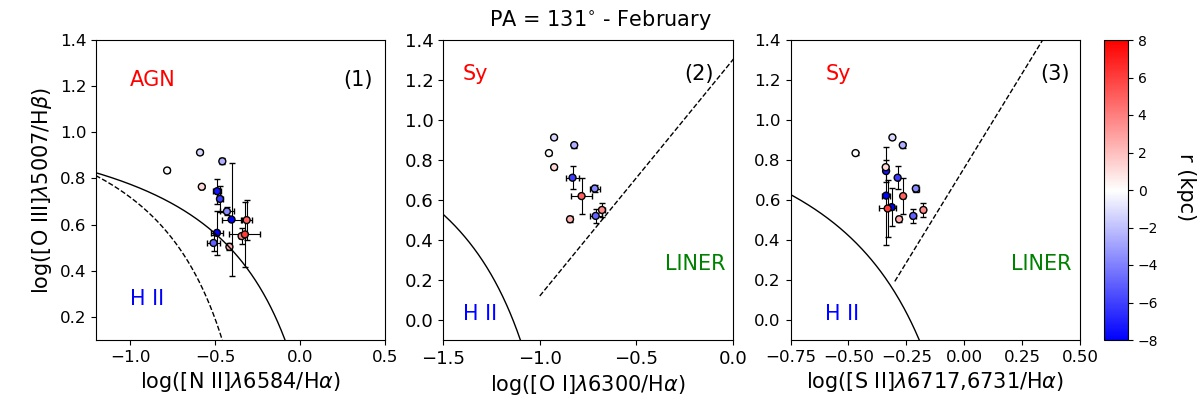
\includegraphics[width=\textwidth]{images/paper3/PA90_diagnostic.jpg}\\ 
\caption[]{Diagnostic diagrams for the LDSS-3 spectra. From top to bottom February PA $=\ang{131}$, June PA $=\ang{131}$ and June PA $=\ang{90}$. For each spectrum the left panel is the  $\log [\rm \ion{O}{III}]\lambda5007/\Hb$ vs $\log [\rm \ion{N}{II}]\lambda6584/\Ha$ diagram, the central panel the $\log [\rm \ion{O}{III}]\lambda5007/\Hb$ vs $\log [\rm \ion{O}{I}]\lambda6300/\Ha$ diagram while the right panel is the $\log [\rm \ion{O}{III}]\lambda5007/\Hb$ vs $\log [\rm \ion{S}{II}]\lambda\lambda6717,6731/\Ha$. The colorbar shows, for each point, the distance from the nucleus of the corresponding spectrum.
In each panel, the solid curve is the \citet{Kewley01} relation dividing AGN from star forming region, the dashed curve is the \citet{Kauffmann03} line for pure star formation while the dashed lines are the \citet{Kewley06} relations dividing Seyfert galaxies from LINERs.
The error bars represent $1\sigma$ errors on the line ratios. Where they are absent, the dimension of the bars is smaller than the size of the corresponding point. 
}
\label{fig:pap3_diagnostic}
\end{figure} 

Fig.\,\ref{fig:pap3_diagnostic} shows the aforementioned diagnostic diagrams for the three LDSS-3 spectra.
The plots show that the main ionization mechanism of the gas is photo-ionization by the AGN.
So, at least for the inner $\sim 8\,\si{kpc}$ the extended emission actually is the ENLR of the AGN.
However, there are some points in the $\log [\rm \ion{O}{III}]\lambda5007/\Hb$ vs $\log [\rm \ion{N}{II}]\lambda6584/\Ha$ diagram that are located in the region between \citet{Kewley01} and \citet{Kauffmann03} lines.
This means that there might be some star forming regions contributing to the ionization of the ISM.
It is interesting to notice that the position of the points in the diagnostic diagrams of the two PA $=\ang{131}$ spectra are quite different, meaning that probably they are observing slightly different regions because of a slightly different alignment. 

In the analysis of these plots, it must be considered that the subtraction of the stellar continuum has not been performed.
This might produce an overestimate of the diagnostic ratios, at least in some spectra.
Therefore, it is possible that the subtraction of the stellar continuum might move some other points in the mixed region or shift some of the point already in this region into the \ion{H}{II} one.
However, the global results should not change much, and the AGN is the main ionizing source of the gas, at least up to a distance of the order of $\sim 10\,\si{kpc}$.

From Fig.\,\ref{fig:line_fluxes} it is possible to see that, at PA $=\ang{131}$ the limiting lines are the low ionization forbidden lines ([\ion{N}{II}], [\ion{S}{II}] and [\ion{O}{I}]) while at PA $=\ang{90}$ is $\Hb$ the missing line at high distances from the nucleus.
Therefore, it is still possible to use the $\log[\rm \ion{O}{III}]\lambda5007/\Hb$ ratio to estimate the ionizing source of some of the most distant regions at PA $=\ang{131}$ and  $\log[\rm \ion{N}{II}]\lambda6584/\Ha$ in the remaining spectrum.
A $\log[\rm \ion{O}{III}]\lambda5007/\Hb>0.6$
guarantees a classification as AGN in two out of three diagnostic diagrams while $\log[\rm \ion{n}{II}]\lambda6584/\Ha$ should be greater than $-0.5$ to tentatively classify the region at least as a mixed ionization zone in the left panels of Fig.\,\ref{fig:line_fluxes}.
In order to classify a region as ionized by the AGN with only the $\log[\rm \ion{n}{II}]\lambda6584/\Ha$ ratio, the measured value should be greater than $-0.1$.

Fig.\,\ref{fig:o3hb_ratio} shows the above mentioned plots.
From the top and middle panels it is possible to see that most of the regions at PA $=\ang{131}$ are ionized by the AGN also at high distances from the nucleus, since most of the points are above the $\log[\rm \ion{O}{III}]\lambda5007/\Hb=0.6$ limit.
On the other hand, in the bottom panel no points fell above the $\log[\rm \ion{n}{II}]\lambda6584/\Ha=-0.1$ limit, and most of them are in the section of the plot enclosed between the two limits.
However, it is clear form the diagnostic diagrams in Fig.\,\ref{fig:pap3_diagnostic} that low [\ion{n}{II}]$\lambda6584/\Ha$ values do not mean that the region cannot be ionized by the AGN, but only that this ratio is not sufficient to realistically estimate the ionizing source of the gas.


\begin{figure}
\centering
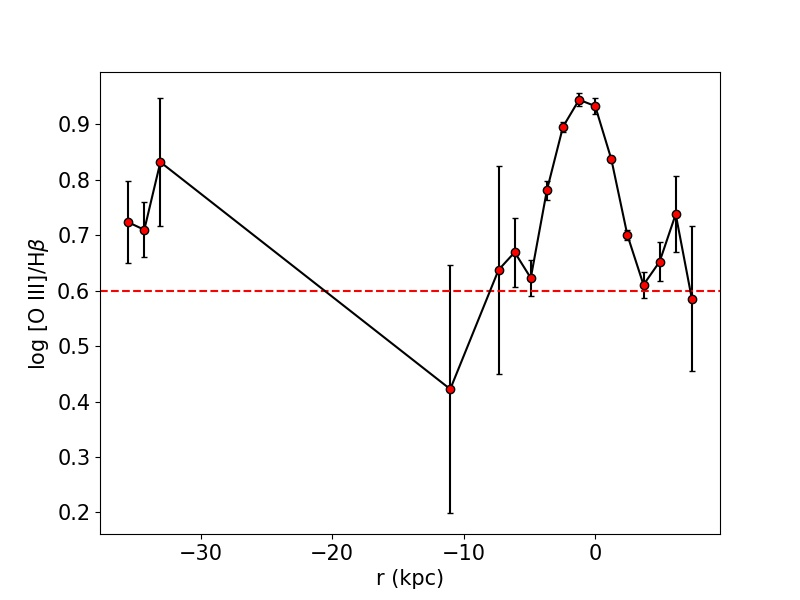
\includegraphics[width=0.6\textwidth]{images/paper3/PA131_2016_o3_hb.jpg}\\ 
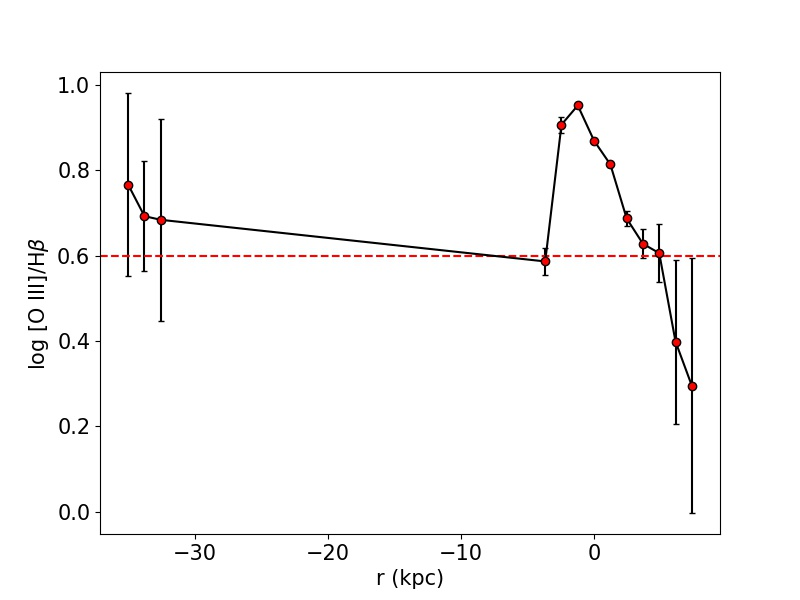
\includegraphics[width=0.6\textwidth]{images/paper3/PA131_o3_hb.jpg}\\ 
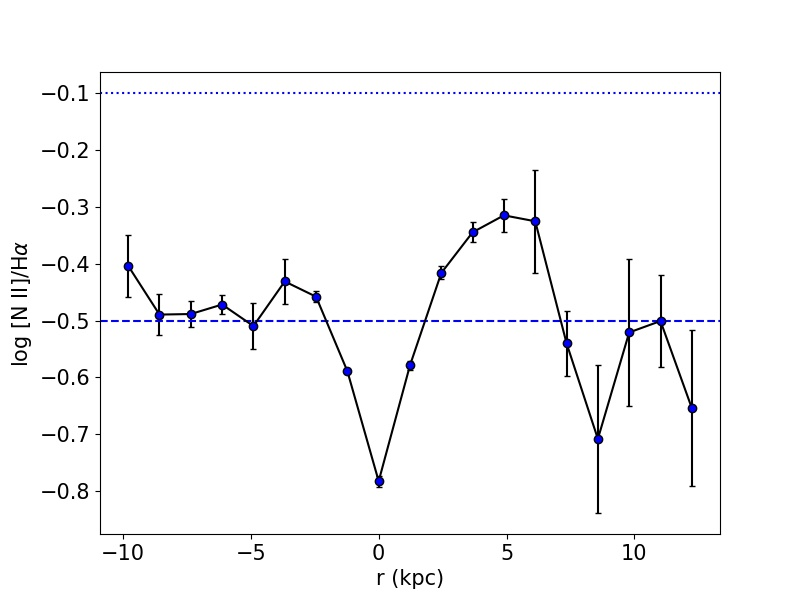
\includegraphics[width=0.6\textwidth]{images/paper3/PA90_n2_ha.jpg}\\ 
\caption[]{\textbf{Top:} $\log [\ion{O}{III}]\lambda5007/\Hb$ vs distance from the nucleus plot for February PA $=\ang{131}$ spectrum. The dashed line represents the $0.6$ limit.
\textbf{Middle:} same plot as the previous panel for June PA $=\ang{131}$ spectrum.
\textbf{Bottom:} $\log [\ion{n}{II}]\lambda6584/\Ha$ plot for June PA $=\ang{90}$ spectrum. In this plot the dashed line represent the $-0.5$ limit for mixed ionization and the dotted line is the $-0.1$ limit for AGN ionization. As in the diagnostic diagrams, the error bars represent $1\sigma$ error on the line ratios. Absent bars means that they are smaller than the size of the point.}
\label{fig:o3hb_ratio}
\end{figure} 


\section{Discussion}
\label{sec:pap3_discussion}

The data analyzed in this work have been acquired as a follow up of the source after the discovery of a peculiar kiloparsec-scale radio emission region (KSR).
The main question is, therefore, if there is a connection between the KSR and the ENLR of Mrk 783.
An important clue of a connection is that the most extended part of the ENLR has been found perfectly aligned with the most extended lobe of the radio emission.
According to \citet{Wilson94} it seems that the relativistic jet launched by the AGN is able to clear the path of the ionizing radiation in the ISM.
This might be what happened in Mrk 783.
Even though the radio emission is a relic, as suggested in \citep{Congiu17}, the original radio jet might have been able to clear the path for the radiation, allowing it to reach larger distances with respect to what happens in other ENLR.
However, the size of the KSR is less than half the extension of the ENLR at the same position angle.
Fig\,\ref{fig:map} shows how the bulk of the radio emission is located inside the nucleus of the galaxy, even though the jet might have been able to dig in the most dense part of the ISM.
Fig\,\ref{fig:map} also shows how the emission on the north-west side of the nucleus is only visible applying a taper to the image, in agreement with the fact that the optical emission in that region is less extended.
On the other hand, no particularly extended radio emission is observed at PA $=\ang{90}$, while the ENLR there reaches a size of $17.5\,\si{arcsec}$.
Since the morphology of the ENLR is not known, it is not possible to definitively confirm that the axis of the two extended regions are aligned.
Narrow-band images or integral field spectra would be necessary to investigate this topic.

%The temperature of the gas in the regions close to the nucleus of the AGN seems to be higher than the typical temperature of photo-ionized regions ($10000$--$20000\,\si{K}$), but it is in agreement with the results of \citet{Vaona12}.
%It is possible that shocks are contributing to the heating of the gas, but they do not have a major role.

Besides the relation with the radio emission, the data analyzed in this work confirmed that Mrk 783 is a very peculiar object.
Firstly, the ENLR observed in this source, with a maximum size of $\sim 38\,\si{kpc}$, is one of the largest discovered so far in the nearby universe and it is located in a Type 1 object, which are believed to host smaller ENLR \citep{Schmitt03b} with respect to Type 2 objects.
There are a few sources with similar ENLR sizes UGC 7342 and NGC 5972 \citep[$37$ and $33$ kpc respectively][]{Keel12} but ENLRs larger than $30\,\si{kpc}$ are usually observed only in objects at $z>0.1$ \citep[e.g.][]{Stockton87,Humphrey10,Sun18}.

Both UGC 7342 and NGC 5972 show a disturbed morphology and UGC 7342 is and ongoing merger.
Since the gravitational interaction produced during a merger influences the gas distribution, it is possible that it can creates the conditions needed to produced larger ENLR than in stable systems.

The analyzed data show several properties of Mrk 783 suggesting that it recently merged with another object.
The extended structure observed in the SDSS and AFOSC images resemble the tidal tails observed in interacting systems like the Antennae galaxies.
A secondary nucleus is observed and in Sec.\,\ref{sec:morph_color} several scenario for its origin has been analyzed and most of them involve a merging episode.
Finally, the complex kinematics shown in Fig.\,\ref{fig:velocity_lines} might be a consequence of the merging event, meaning that the episode happened no more than $\sim 0.4\,\si{Gyr}$ ago, which is the limit after which the kinematical signature of a merging should be no longer observable.
The spectral and spatial resolution of the data are not high enough neither to detect multiple kinematical components in a single region, nor to investigate where is located the dynamical center of the galaxy, to identify which one between the AGN and the secondary nucleus is the real nucleus of the galaxy.
However, there are several hints suggesting that Mrk 783 might have merged with a companion galaxy, and the merging event could be the reason of the large extension of the ENLR.

In support of the merging hypothesis there is also the discovery of the companion galaxy J1302+1625 $\sim100\,\si{kpc}$ away from the nucleus of Mrk 783 which proves that Mrk 783 is not an isolated object.
The two galaxies are also close enough that they might be in the early phases of interaction.

It might also be possible that the merging event that produced the disturbed morphology of the object is also responsible for the ignition of the AGN.
Merging events are now widely accepted as one of the few mechanism that are able to bring gas close to the supermassive black hole of a galaxy, supplying it of the gas needed for the accretion \citep{Sanders88,Hong15}.
Moreover, according to \citet{Mathur00}, NLS1 resides in rejuvenated galaxies, that is galaxies where new gas has been accreted following a galaxy-galaxy merging.

The morphology of Mrk 783 ENLR, instead, is still unknown.
The orientation of the cone and the gas distribution cannot be determined without, at least, a narrow band image of the [\ion{O}{III}]$\lambda5007$ line emitted by the gas.
One of the few things that can be observed from the spectra is that in each long slit spectra the emission is extended on both sides of the nucleus, but one side is always more extended than the other.
The typical shape of the ENLR is that of a bi-cone \citep{Pogge88,Schmitt94,Fischer13} and usually, because of its inclination with respect to the galaxy disk, one of the sides is more extended than the other because of extinction due to the dust present in the disk.
The light of the cone beyond the disk must cross a larger amount of gas and dust than the other cone, and it often results shorter \citep[e.g. NGC 5643,][]{Simpson97} or, in some cases, absent \citep{Wilson96}.

From the PA of the spectra it is possible to give a rough estimate of the opening angle of the ionization cones.
Assuming that the more extended part of the spectra at PA $=\ang{131}$ and PA $=\ang{90}$ belongs to the same cone, it is possible to estimate a minimum opening angle of $\sim 139\,\si{arcsec}$, which is quite large but not outside the possible values found by \citet{He18}.
On the other hand, if the more extended regions are part of opposite cones, the minimum opening angle is reduced to $41\,\si{arcsec}$.

Fig.\,\ref{fig:three_spectra} shows that the extended emission at PA $=\ang{131}$ is not continuous but it seems that the most extended emitting region is separated from the main galaxy.
From the images it is not clear the nature of this emitting region, it can be both a single cloud of part of a faint tidal tail.
A peculiar property of this region is the absence of emission lines of low ionization ions ([N II], [S II]), even though the SNR of some of the extracted spectra is high enough for them to be detected.
This might be an indication of the very high ionization of the gas in this particular region.


\section{Summary}
\label{sec:pap3_summary}

In this work I analyzed new optical data of the NLS1 galaxy MRk 783.
The object shows an extended narrow line region with a maximum extension of $\sim 38\,\si{kpc}$ projected.
The position angle of the maximum extension of the ENLR corresponds to the position angle of the maximum extension of the KSR discovered by \citet{Congiu17}.
Diagnostic diagrams and other line ratios confirm that the ionizing source of the gas in most of the regions analyzed is the AGN itself.

The galaxy also shows peculiar spectral properties that require new data and a dedicated analysis to be properly studied.
Its morphology is disturbed and a secondary nucleus is observed, probably the consequence of a quite recent merging, as suggested by the complex rotation curves observed from $\Ha$ and [\ion{O}{III}]$\lambda5007$.

The object, therefore, is one of the most interesting AGN with ENLR discovered so far.
Unfortunately, the data gathered up untill now are insufficient to have a complete picture of the properties of Mrk 783.
Narrow band images and integral field spectroscopy will be fundamental resources to improve our knowledge on this object.
Understanding the relation between the ENLR and the radio emission, the merging events and all the other properties of this galaxy will be of the uttermost importance to shred light on the feedback processes between the AGN and its host. 

A wider study to detect and characterized other similar object will be fundamental to understand if Mrk 783 is only a ``lucky case'' and what is its position in the class of NLS1 and AGN in general. 



























\biblio
\end{document}